\chapter{Selección de eventos: definición de las regiones de señal}
\label{cap:seleccion}

Como se discutió en la \cref{sec:regiones}, las regiones de señal son un
componente clave del análisis dado que son aquellas en las que se espera la
presencia de eventos de nueva física. En este capítulo se describe la selección
de eventos que define las regiones de señal del análisis de esta tesis. Esta
selección fue optimizada en base a la significancia esperada de descubrimiento
utilizando las muestras MC de señal y fondos del SM.


\section{Criterios de calidad sobre los datos}

%% GRL: data12_8TeV.periodAllYear_DetStatus-v61-pro14-02_DQDefects-00-01-00_PHYS_StandardGRL_All_Good.xml

Para este análisis se ha utilizado una GRL que, además de aplicar requerimientos
generales sobre la operación del experimento y la estabilidad del haz en el
acelerador, contiene aquellos eventos donde todos los subdetectores se
encontraban funcionando en su plena capacidad.

Adicionalmente se eliminan los eventos que contengan algún tipo de problema,
como ruido en el calorímetro, o celdas no operativas, que pueda resultar en
energía faltante instrumental.


\section{\emph{Trigger}}\label{sec:trigger}

Los datos fueron recolectados utilizando un \emph{trigger} de un fotón (\trigchain), que
selecciona eventos con al menos un fotón \emph{loose} con momento transverso mayor a
120 \gev.

La eficiencia de este \emph{trigger} fue calculada utilizando el método \emph{bootstrap}
siguiendo las prescripciones descriptas en \cite{ATLAS-CONF-2011-114,Damazio:1609629}.
Cuando se calcula la eficiencia del \emph{trigger} utilizando el método \emph{bootstrap}, se factoriza
la eficiencia como el producto de la eficiencia del EF respecto a la eficiencia del L1
por la eficiencia de la selección de L1.
La eficiencia de {\trigchain} respecto a fotones aislados con $\pt>125\gev$ resulta en
$100^{+0}_{-1.41}\stat \, {}^{+0}_{-0.7}\syst \%$.

En la \cref{fig:trigger_perf} se puede ver el resultado como función del {\pt}
del fotón.
A pesar de la escasa estadística, es claro que la eficiencia alcanza una meseta,
en la cual la eficiencia es máxima, antes de $125 \gev$. La incerteza total
tiene en cuenta la limitada estadística de la muestra de datos y también la
incerteza en la corrección debido a la pureza de los fotones. El desempeño del
\emph{trigger} se mantuvo estable durante todo el período de la toma de datos
considerado.

\begin{figure}[!htb]
  \centering

  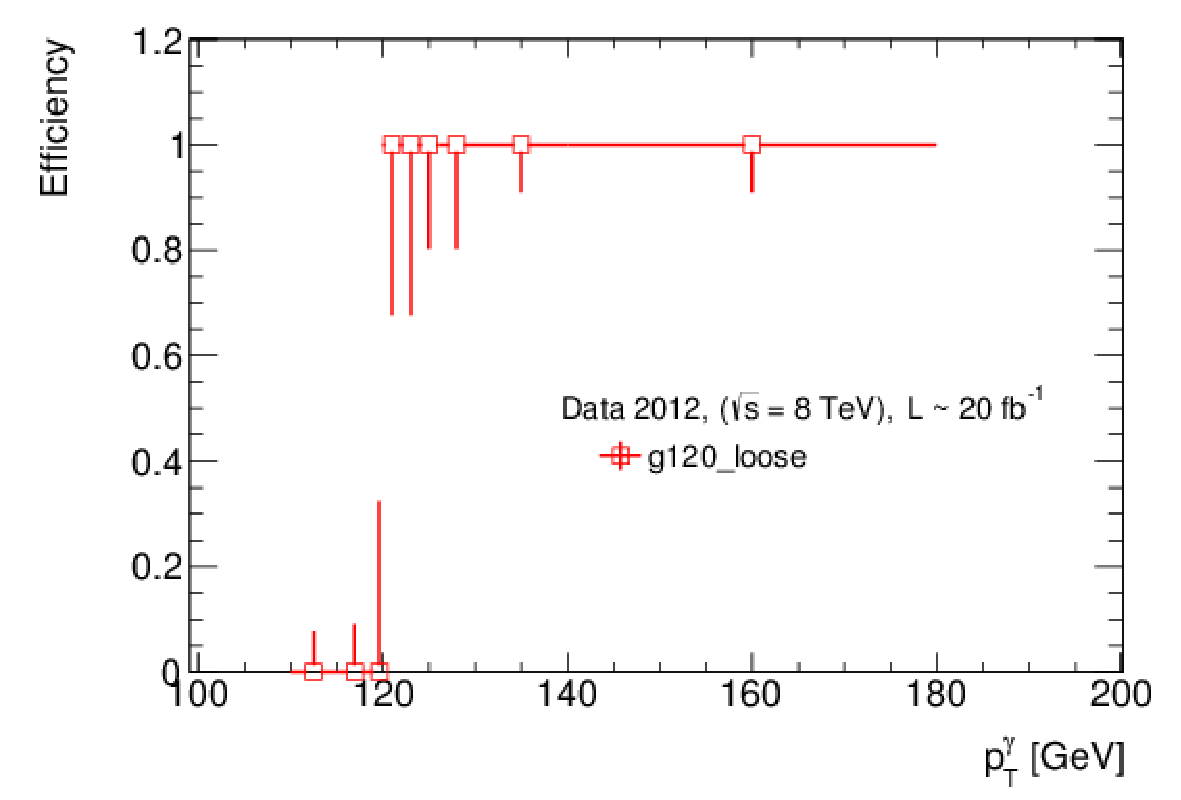
\includegraphics[width=0.6\textwidth]{EffPtg120_loose}

  \caption{Eficiencia del \emph{trigger} {\trigchain} como función del {\pt} del fotón.}
  \label{fig:trigger_perf}
\end{figure}


\section{Preselección}
\label{sec:base_seleccion}

\subsection{Vértice primario}

Como se describe en la \cref{sec:obj_vertex} los candidatos a vértices de la interacción $pp$ son
reconstruidos en cada evento utilizando las trazas en el detector interno. El
vértice primario, correspondiente a la interacción dura de dispersión, es el
candidato con la mayor suma de $p_{\mathrm{T}}^{2}$ para las trazas asociadas. Solo se
consideran los eventos donde el vértice primario tiene al menos cinco trazas
cargadas.


\subsection{Objetos}
\label{sec:preselection}
%% Antes de aplicar los cortes cinemáticos, se realiza la siguiente
%% preselección y limpieza.

En primero lugar se realiza una preselección de los objetos que se consideran en cada
evento como se detalla a continuación y se resume en la \cref{tab:base_sel}. Se
consideran fotones todos aquellos candidatos a fotón que pasen el criterio de
identificación \emph{tight}, que tengan $\pt>75\gev$ y $|\eta|<2.37$. Se
consideran electrones los candidatos que pasan el criterio de identificación \emph{medium}, y
que tengan un $\pt>10\gev$ y $|\eta|<2.47$, y muones a aquellos que pasan un criterio de
identificación \emph{loose} con $\pt>6 \gev$ y $|\eta|<2.5$. Para el caso de
jets, se consideran los que tienen $\pt>20\gev$ y $|\eta|<2.8$.


\begin{table}[!htbp]
  \centering

  \caption{Preselección de objetos. Criterio de identificación (ID) y cortes de
    aceptancia (\pt, $\eta$) considerados para cada tipo de partícula. Además
    del límite superior en $|\eta|$, no se consideran en ningún caso los objetos
    que se encuentren en la región entre la zona del \emph{barrel} y las \emph{end-caps} del detector, es
    decir, con $1.37 < |\eta| < 1.52$.}
  \label{tab:base_sel}

  \begin{tabularx}{0.8\textwidth}{LCCC}
    \hline
    & ID & $\pt$ & $|\eta|$ \\
    \hline
    Fotones    & \emph{tight}  & $> 75 \gev$ & $<2.37$ \\
    Electrones & \emph{medium} & $> 10 \gev$ & $<2.47$ \\
    Muones     & \emph{loose}  & $> 6  \gev$ & $<2.5$  \\
    Jets       & -             & $> 20 \gev$ & $<2.8$  \\
    \hline
  \end{tabularx}

\end{table}


%% La selección de los objetos se realiza según lo descripto en \cref{sec:obj_selection}.
%% El overlap removal y el event veto aplicado se detalla en la \cref{sec:overlap_romoval_event_veto}.

%% Excepto durante calculo de {\met}, dos cortes de aceptancia extra son requeridos
%% para los jets: $\pt > 40 \gev$ y $|\eta| < 2.8$.
%% Todos los jets pasando esta selección \emph{loose} son considerados cuando se aplica
%% la identificación de objetos descripta en \cref{sec:overlap_romoval_event_veto}.


\subsection{Eliminación de objetos superpuestos}
\label{sec:overlap_romoval_event_veto}

De acuerdo a las definiciones de objetos presentadas más arriba, un objeto puede estar en
más de una categoría, contándose dos veces. Por este motivo se realiza un
procedimiento para remover este solapamiento, el cual se aplica sobre los
objetos preseleccionados antes de aplicar los criterios de aislamiento. El
procedimiento para remover estas ambigüedades entre los objetos es el que se
detalla a continuación en ese orden:

\begin{itemize}\itemsep0.1cm
\item Si un fotón o electrón se encuentran dentro de $\Delta R < 0.01$, el
  objeto es considerado como un electrón, removiéndose el fotón correspondiente.
  Esta elección reduce la tasa de electrones mal reconstruidos como fotones.
\item Los jets que estén cerca ($\Delta R<0.2$) de un electrón o fotón
  preseleccionado se remueven.
\item Fotones y electrones preseleccionados son removidos si su distancia al jet
  más cercano es $0.2 < \Delta R < 0.4$.
\item Muones preseleccionados son removidos si su distancia al jet más cercano
  es $\Delta R < 0.4$.
\end{itemize}


%% \subsection{Limpieza de eventos}

Por último, para asegurar el correcto cálculo de la energía faltante, y reducir
los eventos con energía faltante instrumental, los eventos que satisfacen
alguna de las condiciones siguientes son descartados.

\begin{itemize}\itemsep0.1cm
\item Si el evento (después de de la preselección de objetos y la eliminación de los objetos superpuestos) contiene al menos
  un jet que falla los cortes de limpieza de jets que se definen en
  \cref{sec:jet_obj}.

\item Eventos con muones cósmicos: cuando el evento tiene al menos un muon con $|z_{0}| > \unit[1]{mm}$ o $|d_0| >
  \unit[0.2]{mm}$, donde estos valores son calculados con respecto al vértice
  primario. %%Estos muones tienen altas posibilidades de ser muones cosmicos \note{Check!}
\end{itemize}

Después de esta limpieza de eventos, con los objetos definidos en las secciones anteriores y después
de haber eliminado los objetos duplicados, se calcula la energía faltante transversa como se explica
en \cref{sec:met_obj}.



\section{Optimización de la selección de las regiones de señal}

Como primer paso se seleccionan eventos que contengan el estado final buscado:
un fotón, al menos un jet y energía faltante, y, a partir de esa selección
inicial, se eligen observables que permitan separar la señal del fondo y se
optimizan los cortes en estos observables.

Del estudio realizado en la \cref{sec:susy_studies}, resultan evidentes las diferencias
cinemáticas y topológicas de los eventos en las distintas regiones del
espacio de parámetros {\mgmn} del modelo de SUSY.
Es por esta razón que resulta conveniente tener más de una región de señal,
cada una destinada a una zona particular del espacio de parámetros.

Por tal motivo, se dividió el análisis en dos regiones de señal, a las que se
llamó {\SRL} y {\SRH}. La primera de ellas, \SRL, se focaliza en la zona en la que
los gluinos decaen en cascada hasta neutralinos NLSP de baja y
moderada masa. Los eventos de señal en esta región se caracterizan por una gran
multiplicidad de jets y actividad hadrónica, debido a que involucra cadenas de
decaimiento largas de gluinos pesados a través de la producción de charginos y quarks.
Cuanto más baja la masa del {\ninoone}, más baja sera la energía del fotón y
menor es la cantidad de energía faltante. La segunda región de señal, \SRH,
tiene como motivación aquellos escenarios donde la masa del gluino y del neutralino
más liviano están cerca una de la otra. La cadena de decaimiento es por lo tanto
mucho más corta en este caso, con una menor multiplicidad de jets y, debido al
neutralino pesado, fotones de alto {\pt} y gran cantidad de energía faltante en
el estado final.

En la \cref{fig:srs_motivation} puede verse esquemáticamente a que región del espacio
de parámetros de la señal {\mgmn} está destinada cada SR.

\begin{figure}[!htbp]
  \centering
    \resizebox{0.5\textwidth}{!}{
      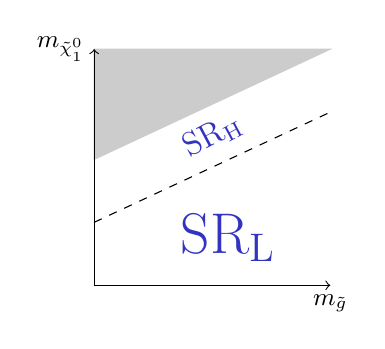
\begin{tikzpicture}

  \colorlet{green}{green!50!black!50}
  \colorlet{red}{red!70!black!50}
  \colorlet{blue}{blue!70!black!80}

  \draw[gray!40,fill] (0, 1.6) -- (3, 3) -- (0,3) -- cycle;

  \draw[->] (0,0) -- (3,0) node[below] {\small $m_{\tilde{g}}$};
  \draw[->] (0,0) -- (0,3) node[left] {\small $m_{\tilde{\chi}_1^0}$};

  %\draw[red,line width=2] (1.5,1.8) circle (15pt);
  \draw[dashed] (0,0.8) -- (3, 2.2);

  \node[blue] at (1.7,0.6) {\huge SR$_{\mathrm{L}}$};
  \node[blue] at (1.5,1.9) [rotate=28] {\large SR$_{\mathrm{H}}$};

\end{tikzpicture}

      }
    \caption{Esquema de la región del espacio de parámetros del modelo de señal en el
    plano {\mgmn} y a que zona esta dirigido el diseño de las dos regiones de señal.}
  \label{fig:srs_motivation}
\end{figure}


Para la optimización de las SR, se utilizaron varios puntos de señal en cada región,
representativos de la topología y el espacio de fase en cada caso:

\begin{itemize}\itemsep0.2cm\parskip0.2cm
\item {\SRL}: $(1150, 200)$ y $(1150, 450)$
\item {\SRH}: $(1150, 850)$ y $(1150, 1050)$
\end{itemize}
%
donde cada punto queda determinado por sus valores $(M_3, \mu)$.

Como fondo se utilizaron las muestras MC, y se consideró una incerteza en la estimación del
fondo de 25\%. Todas las muestras MC fueron normalizadas a una luminosidad total
integrada de 20.3 \ifb. La significancia esperada se calculó utilizando la
\cref{eq:Za}, y para evitar una selección muy restringida, se requiere al menos
un evento de fondo en cada SR. Además de evaluar la significancia esperada para
distintos cortes también se tuvo en cuenta que la eficiencia de señal sea
superior al 20\%.

Los cortes fueron optimizados en el orden de poder discriminatorio, uno a la
vez, y aplicados en el orden descripto a continuación, monitoreando la
significancia para distintos cortes en las variables discriminatorias.

Como ya se ha mencionado, el estado final buscado en este análisis consiste en un
único fotón, jets y energía faltante. Por lo que la definición de las SR
comienza optimizando los cortes en las variables cinemáticas del fotón, los jets
y el corte en energía faltante.

%% Como primer paso se impuso un corte en la energia faltante transversa $\met>150\gev$Se impuso
%% La significancia para cada caso
%% The significance for different cut combinations was also monitored to take the best configuration.
%% A minimal pre-selection cut in $\met>150\gev$ was placed in the SR, which is highly efficient for the signal and very effective
%% removing large part of the SM backgrounds, particularly the QCD multijet production. The final selection requirements are summarised in sec \ref{sec:signal_regions}.



\subsection{Fotón}\label{sec:opt_ph_iso}

El primer paso para definir la SR consistió en seleccionar eventos con un único
fotón de los previamente seleccionados con {\pt} mayor a 125 \gev. Este valor
fue elegido para asegurar la máxima eficiencia del \emph{trigger}.

Los eventos con un segundo fotón con $\pt > 75 \gev$ fueron vetados. El corte en
{\pt} de $75\gev$ fue elegido para que las SR sean ortogonales a las SR del
análisis de ATLAS que busca dos fotones\cite{ATLAS-CONF-2014-001} garantizando la
posible combinación estadística entre ambos. Este análisis fue diseñado para
buscar SUSY en escenarios GGM, pero particularmente en el caso de que el
neutralino NLSP sea mayoritariamente bino, y el decaimiento a fotones sea
dominante.

Como se menciona en la \cref{sec:fotones}, para seleccionar los fotones se
aplica un corte en la energía transversa de aislamiento (\etiso). Específicamente,
para el presente análisis se estudiaron distintos
criterios de aislamiento, variando el tamaño del cono ($R$) en el cual se
calcula esta energía.

En la \cref{fig:photon_iso} se muestran las distribuciones de la energía de
aislamiento para varios valores de $R$ para las muestras de señal en las dos SR.
La SR con mayor diferencia de masa entre gluino y neutralino parece tener
distribuciones más anchas, un efecto que desaparece para tamaños de cono más
chicos. Como se ve en la \cref{fig:photon_iso_sig} (arriba), la mayor eficiencia
de selección se obtiene también para el menor tamaño de cono, $R = 0.2$. Para un
corte de $5 \GeV$, se obtiene una eficiencia alta (85-90\%) a lo largo de toda la
\emph{grid}. Luego de aplicar una preselección en {\met}, los fotones no aislados
provenientes de fondos dominados por procesos QCD son muy suprimidos, reduciendo el impacto
del corte de aislamiento en la significancia.

Incluso luego de que la corrección es aplicada para remover la filtración de
energía del fotón dentro de su propio cono de aislamiento, una dependencia remanente
con el {\pt} del fotón es observada para todos los tamaños de cono
considerados, como se muestra en \cref{fig:photon_iso} (abajo). El tratamiento
de este efecto es discutido en la \cref{sec:jfake_sig_template,sec:expsyst}.


\begin{figure}[!htbp]

  \centering
  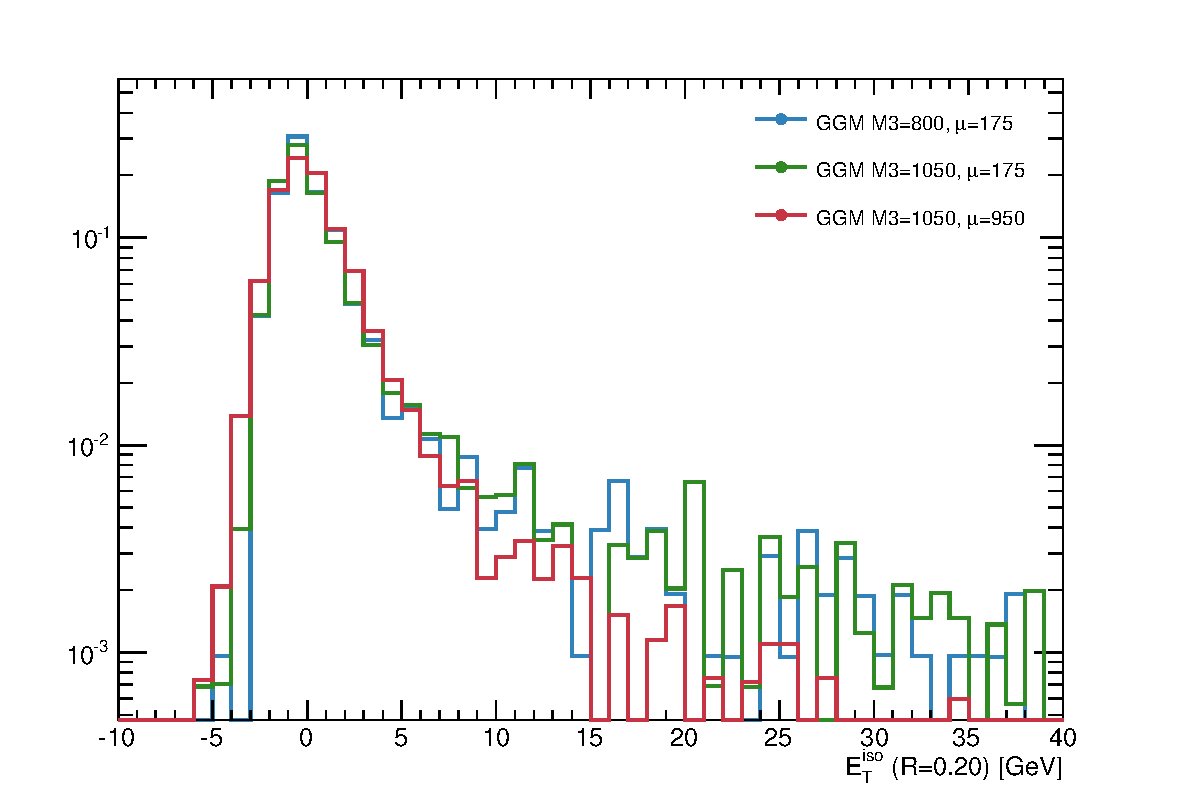
\includegraphics[width=0.32\textwidth]{figures/iso_20}
  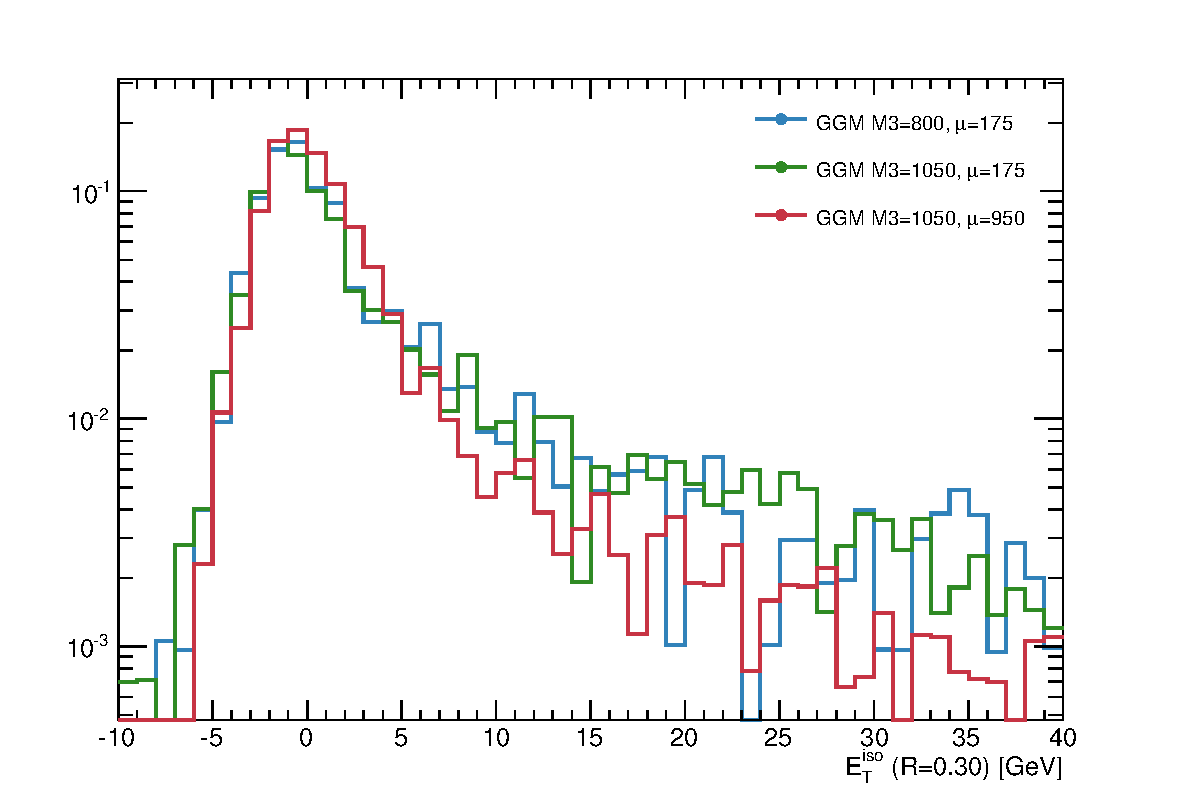
\includegraphics[width=0.32\textwidth]{figures/iso_30}
  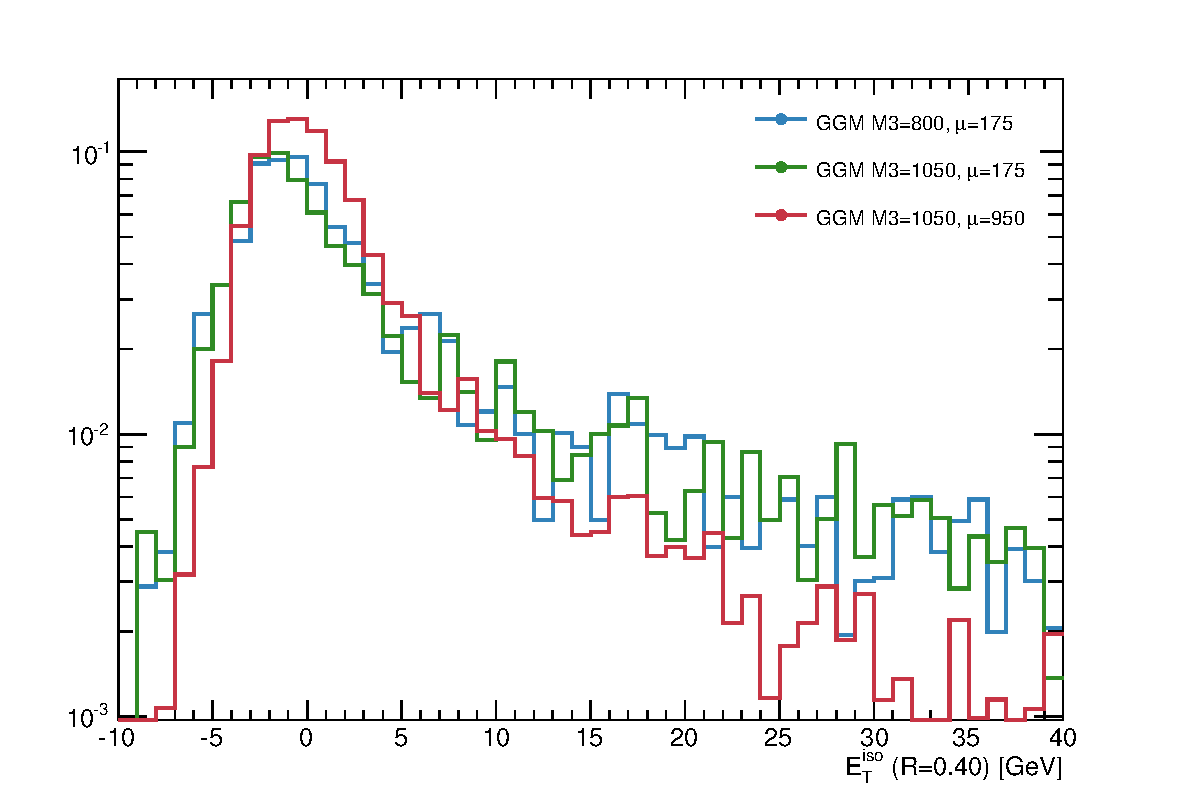
\includegraphics[width=0.32\textwidth]{figures/iso_40}

  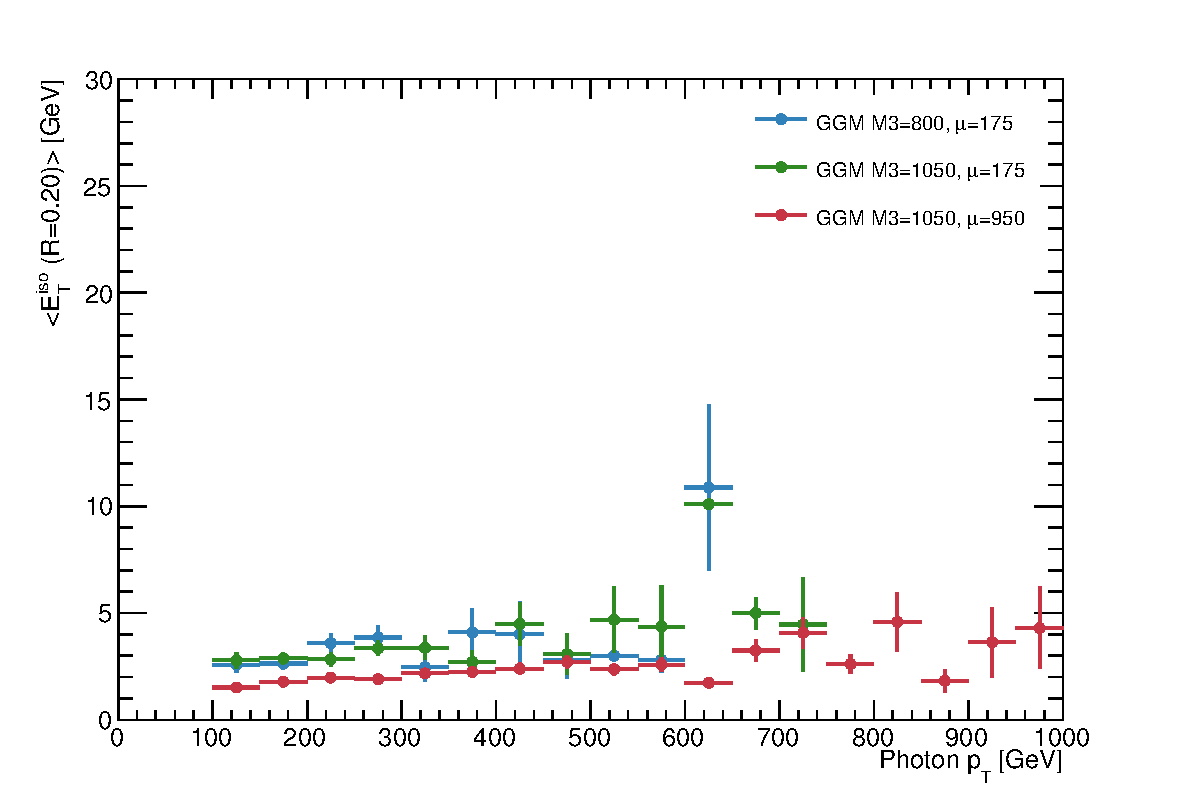
\includegraphics[width=0.32\textwidth]{figures/iso_20_pt}
  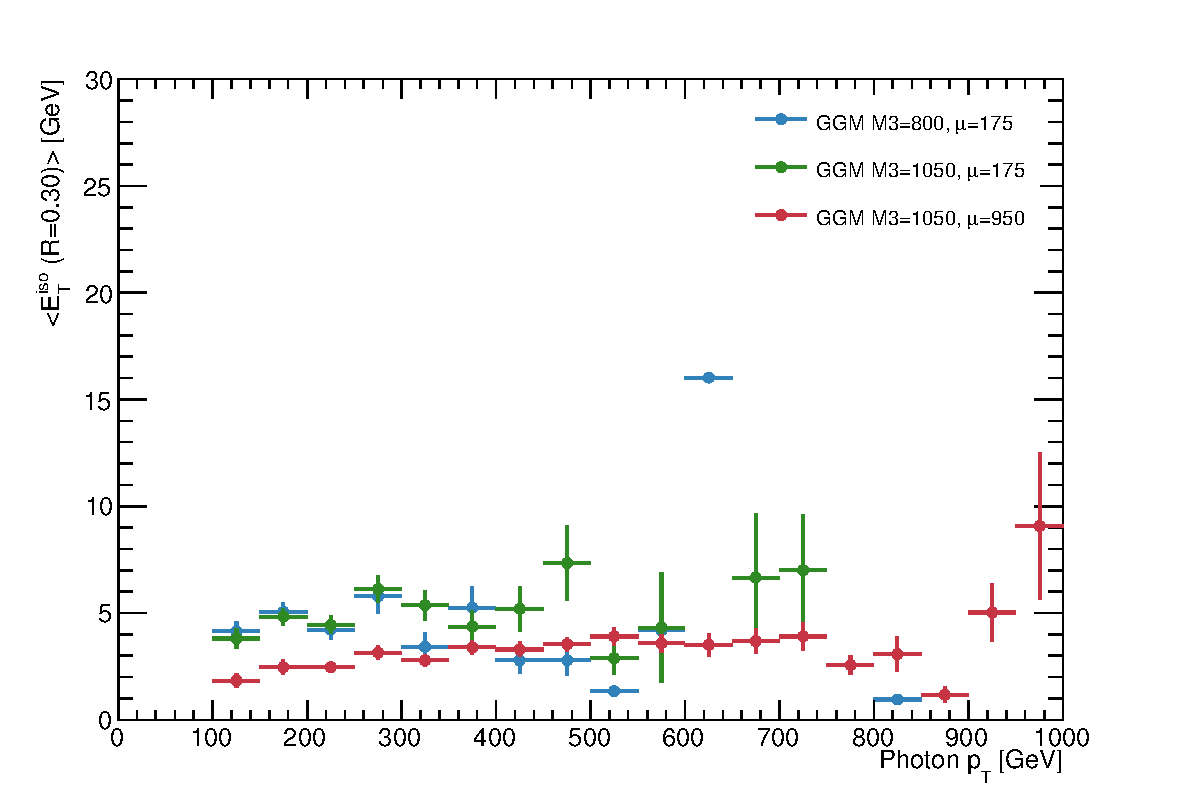
\includegraphics[width=0.32\textwidth]{figures/iso_30_pt}
  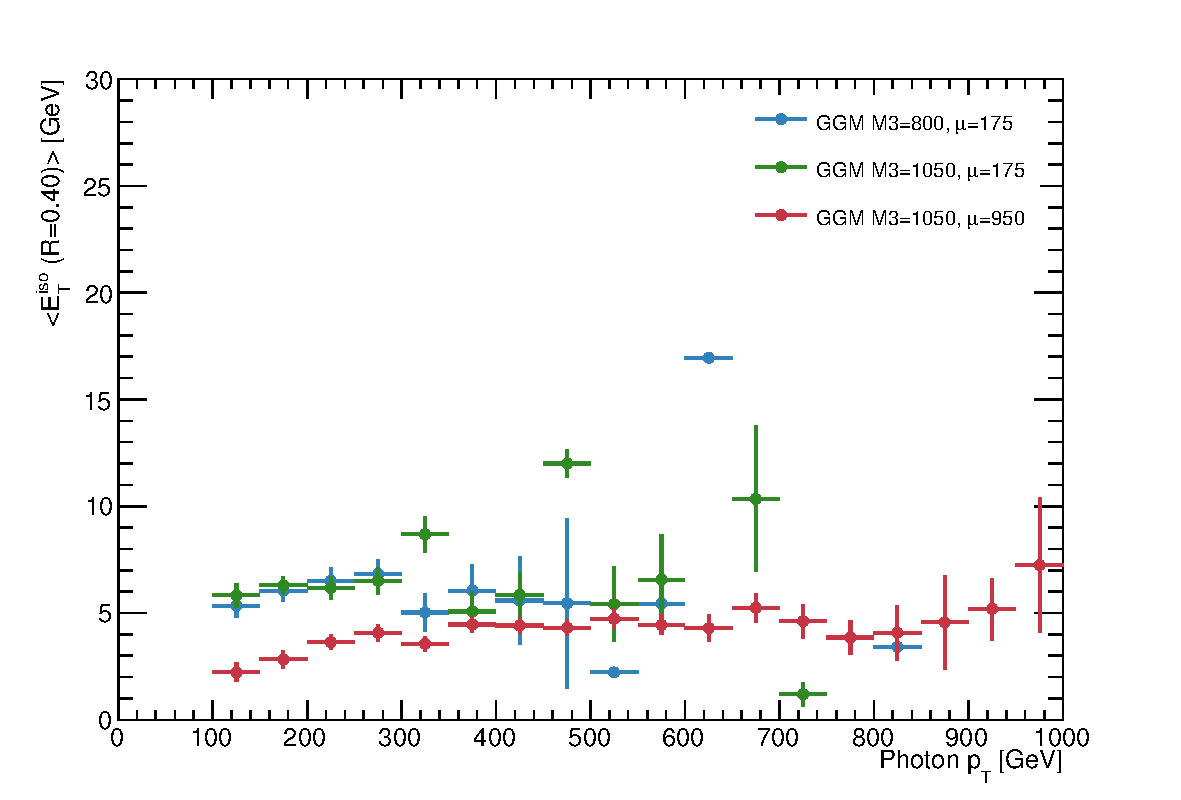
\includegraphics[width=0.32\textwidth]{figures/iso_40_pt}

  \caption{Distribución de {\etiso} (arriba) y su valor medio como función del
    {\pt} del fotón (abajo) para distintos tamaños de conos: $R=0.2$, $R=0.3$ y$R=0.4$.
    Una preselección de $\pt>125\gev$ y $\met>150\gev$ fue aplicada, para suprimir
    gran parte del fondo de fotones directos.}
  \label{fig:photon_iso}
\end{figure}

\begin{figure}[!h]
  \centering

  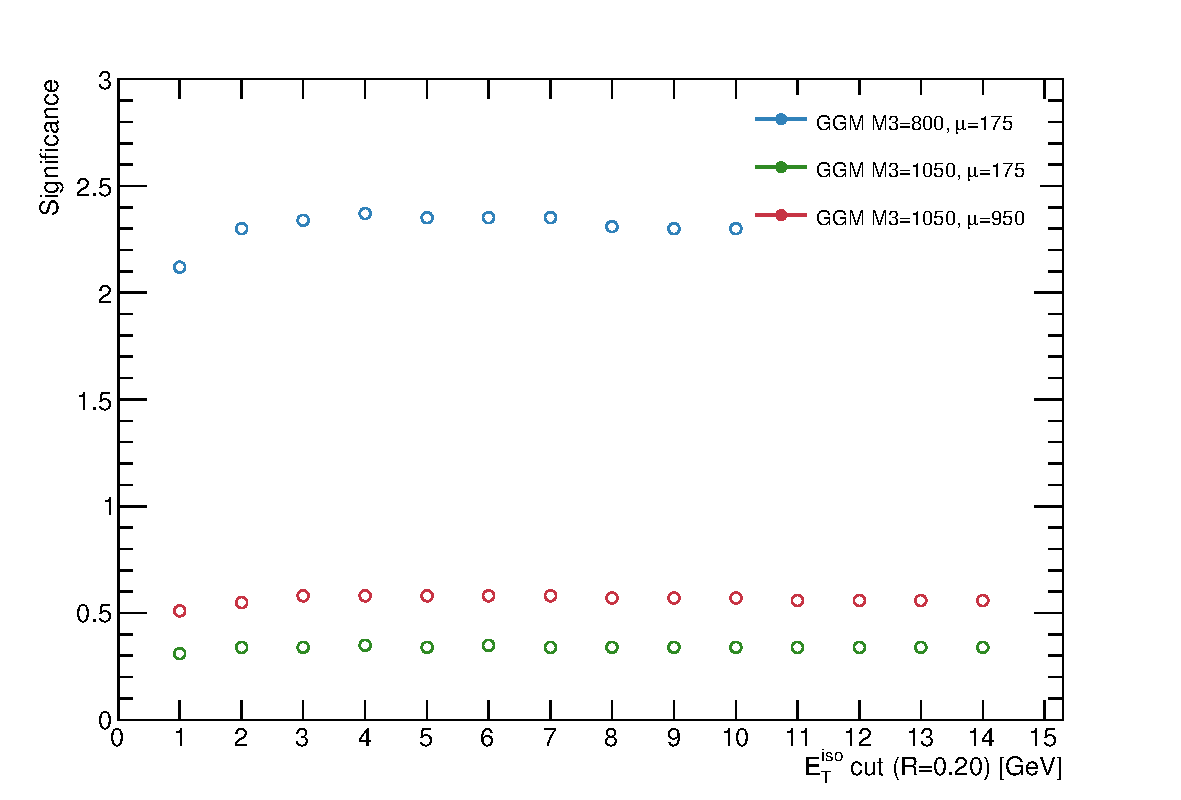
\includegraphics[width=0.3\textwidth]{figures/iso_20_sig}
  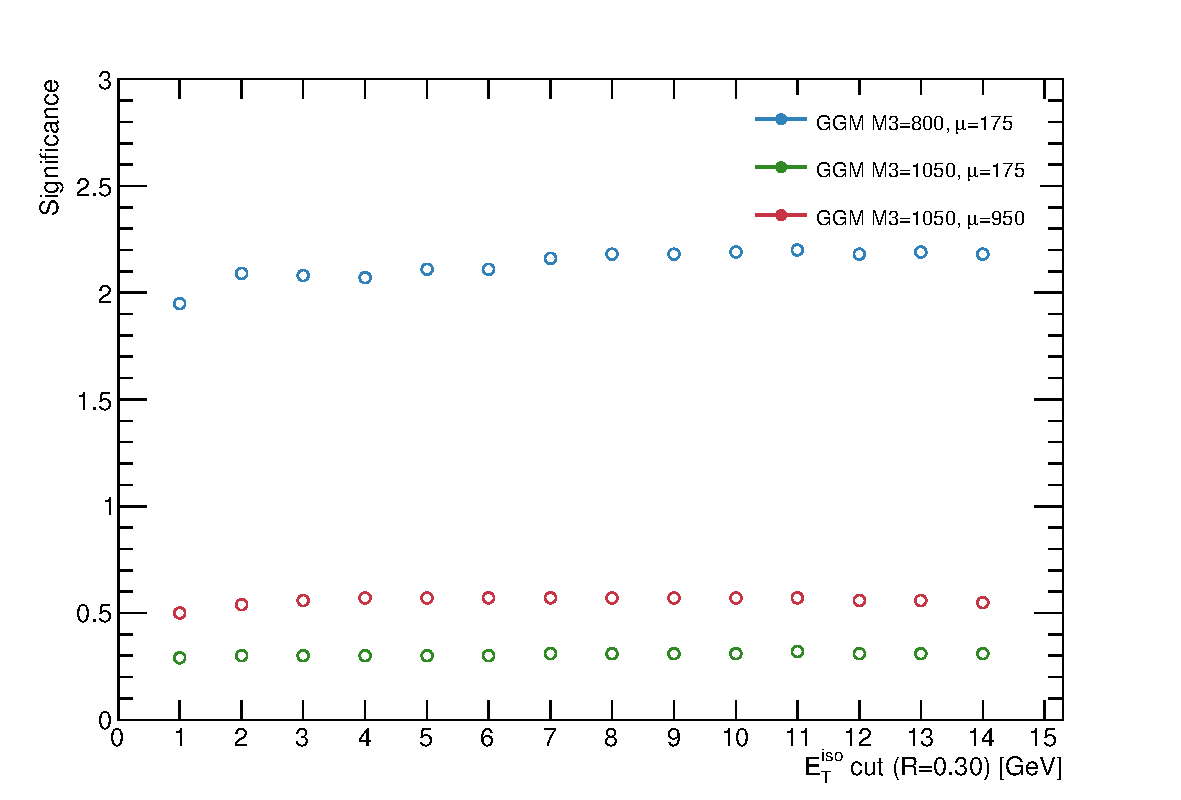
\includegraphics[width=0.3\textwidth]{figures/iso_30_sig}
  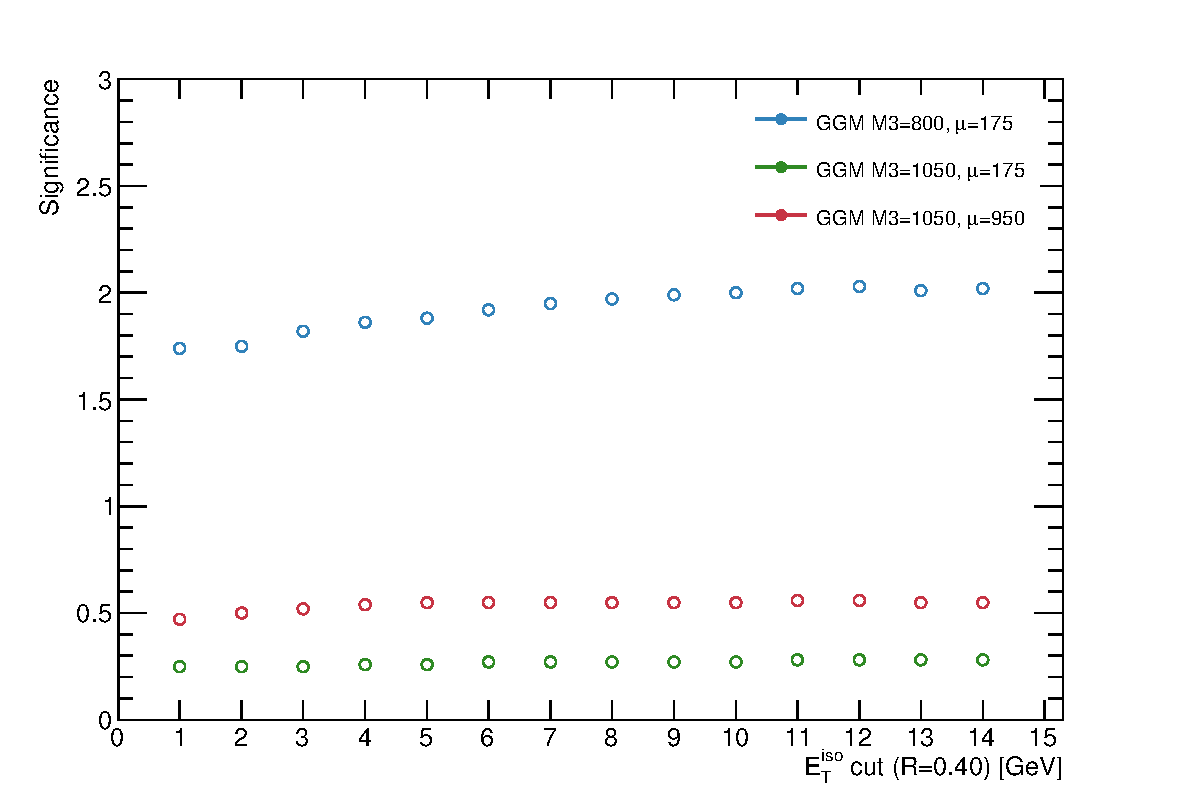
\includegraphics[width=0.3\textwidth]{figures/iso_40_sig}

  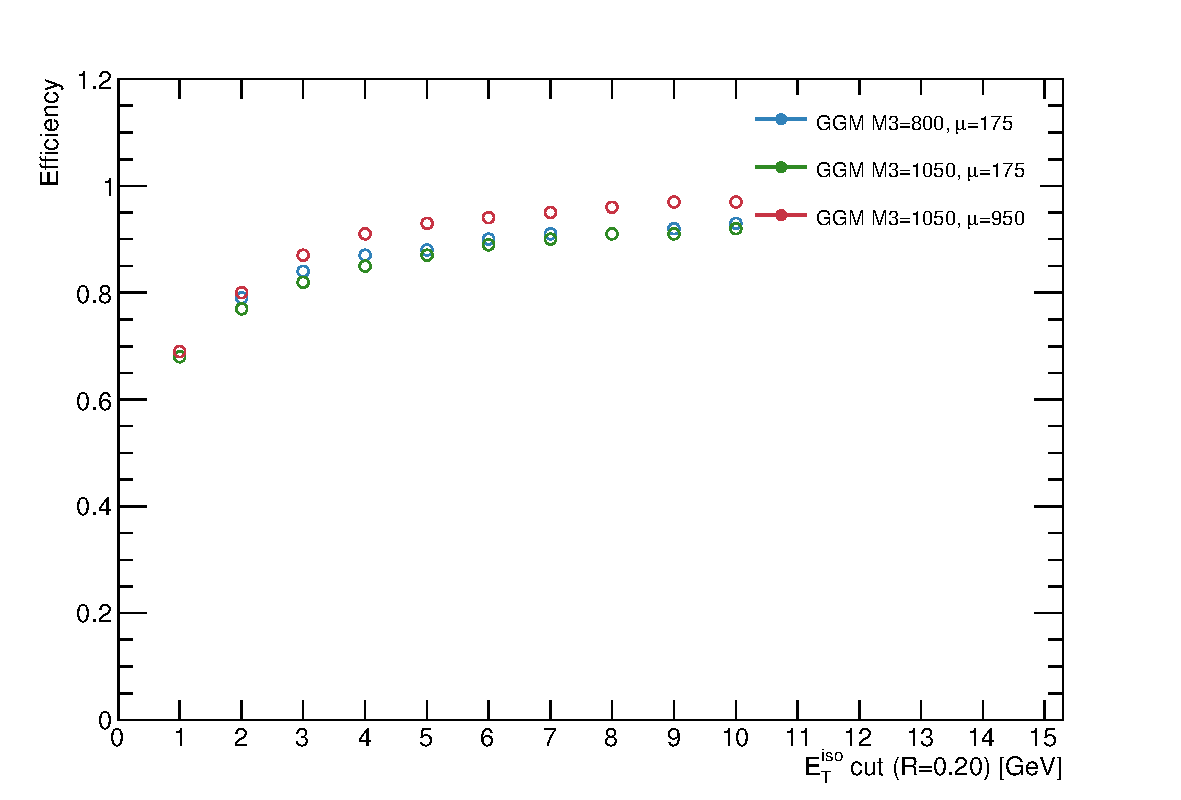
\includegraphics[width=0.3\textwidth]{figures/iso_20_eff}
  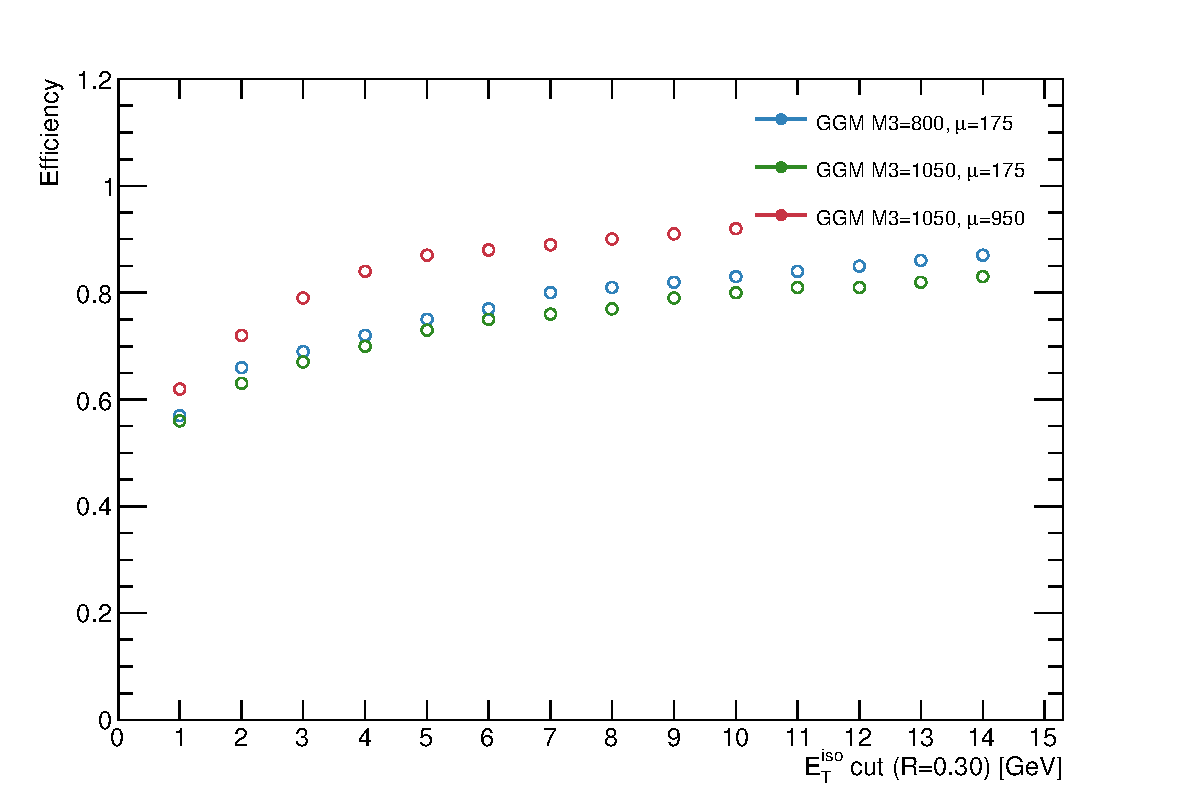
\includegraphics[width=0.3\textwidth]{figures/iso_30_eff}
  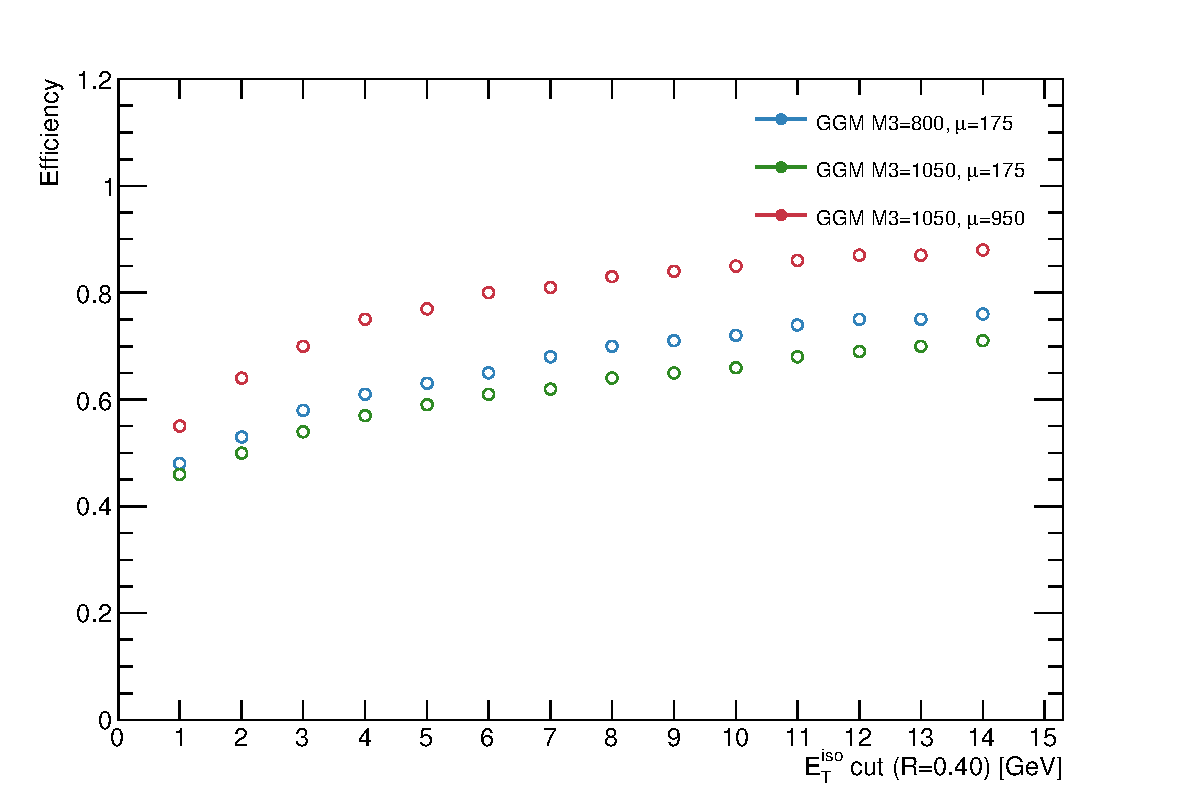
\includegraphics[width=0.3\textwidth]{figures/iso_40_eff}

  \caption{Significancia esperada (arriba) y eficiencia (abajo) como función del
    corte en la energía de aislamiento, después del corte en {\pt} y {\met}.}
  \label{fig:photon_iso_sig}
\end{figure}



\subsection{Leptones}\label{sec:leptonphoton_veto}

Además del veto a los eventos con un segundo fotón, también se remueven
los eventos que contienen leptones ($e$ o $\mu$) con el objetivo de que las
SR no tengan un solapamiento con las SR del análisis que busca estados finales
con un fotón, un leptón y energía faltante \cite{ATLAS-CONF-2012-144}.



\subsection{Energía faltante}

La principal característica de los eventos de SUSY donde se conserva
la paridad-R es la presencia de una gran cantidad de energía faltante debido
a las LSP estables que escapan la detección, en este caso debido a los dos gravitinos
en el estado final.
Un corte en esta variable reduce enormemente la contaminación de procesos
QCD y también de otros procesos del {\SM}.
La \cref{fig:opt_met} muestra la distribución de {\met} en eventos con
un fotón aislado con alto {\pt} (como se definió en la sección anterior),
para dos puntos de señal en cada SR, junto al fondo esperado de simulaciones
MC.

Un corte en {\met} relativamente bajo ($> 200 \gev$) es capaz de separar
la señal y el fondo significativamente en {\SRL}, mientras que para {\SRH}
es posible aplicar un corte más alto ($>300\gev$).

\begin{figure}[!h]
  \centering
  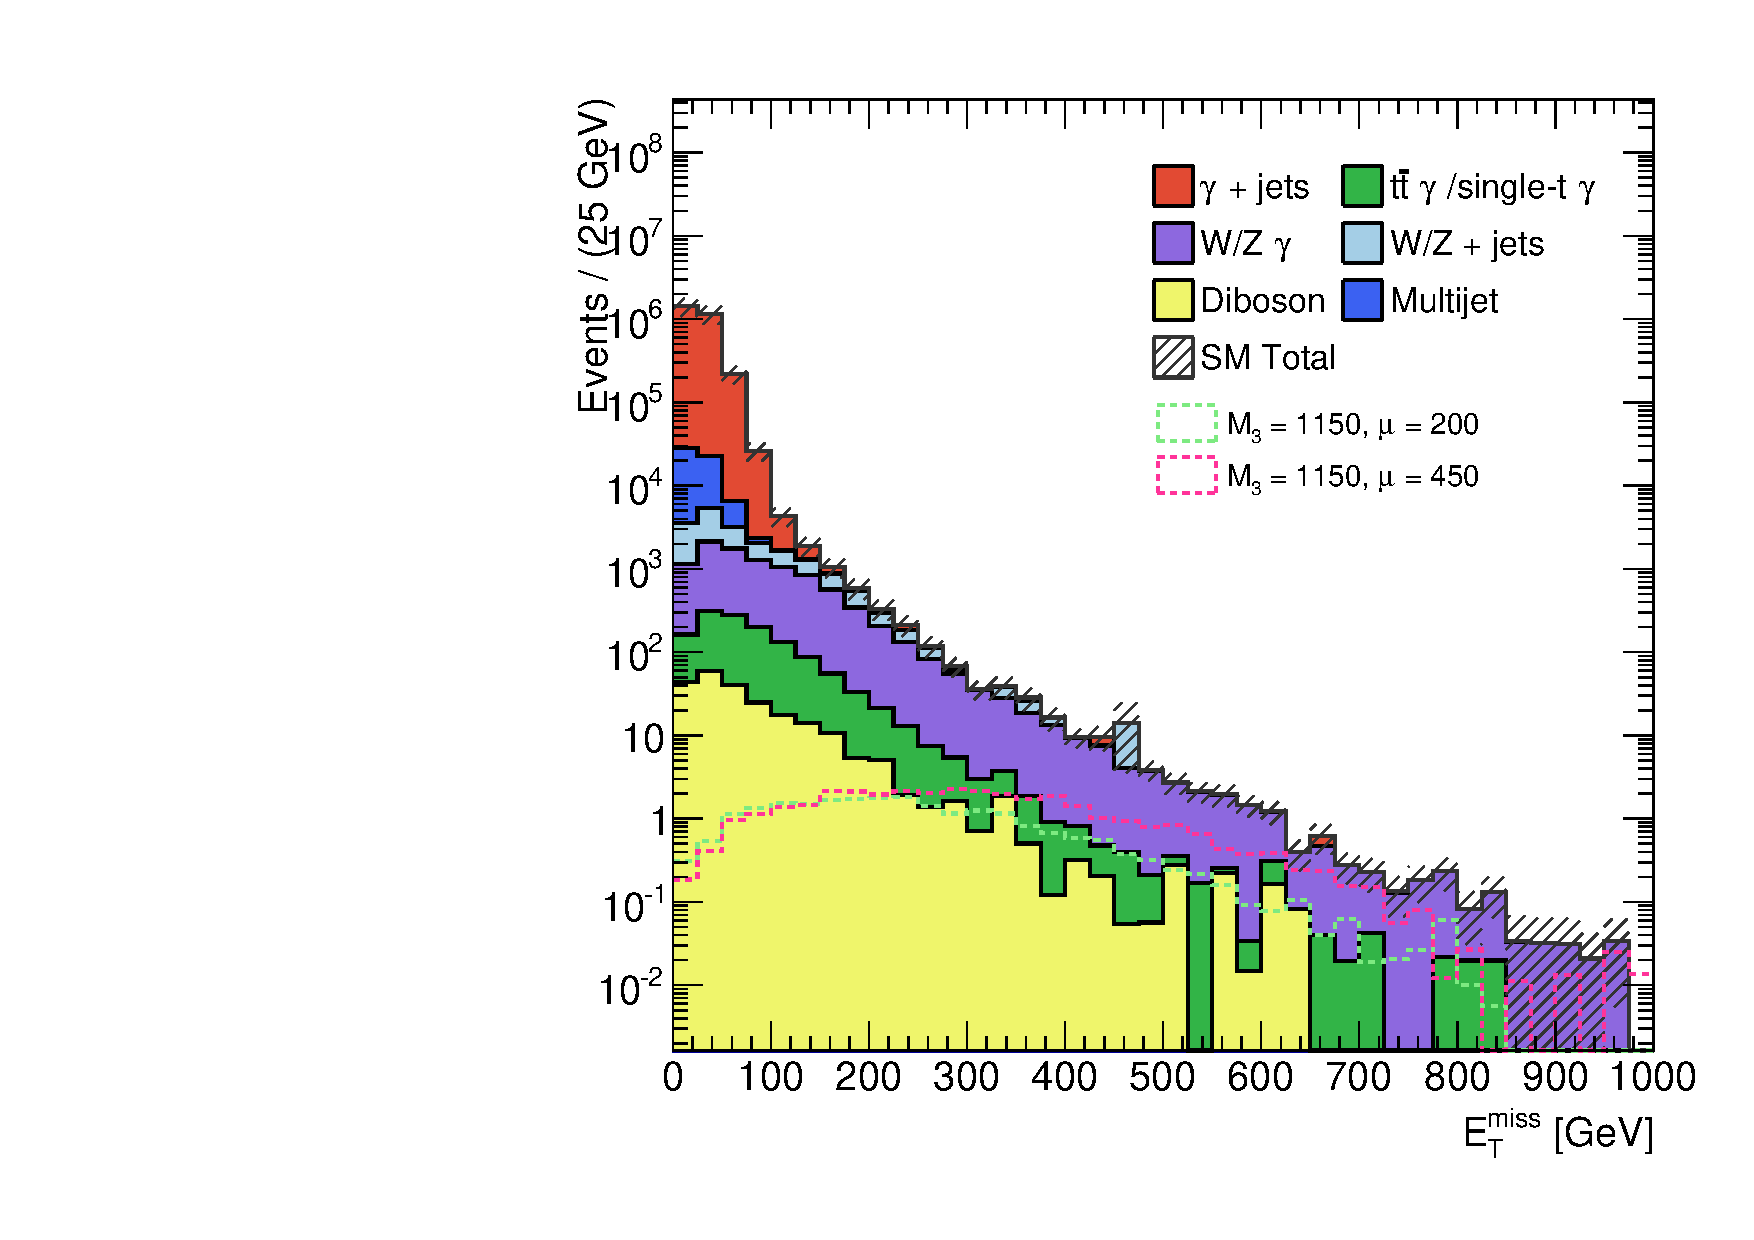
\includegraphics[width=0.49\textwidth]{met_et_base1}
  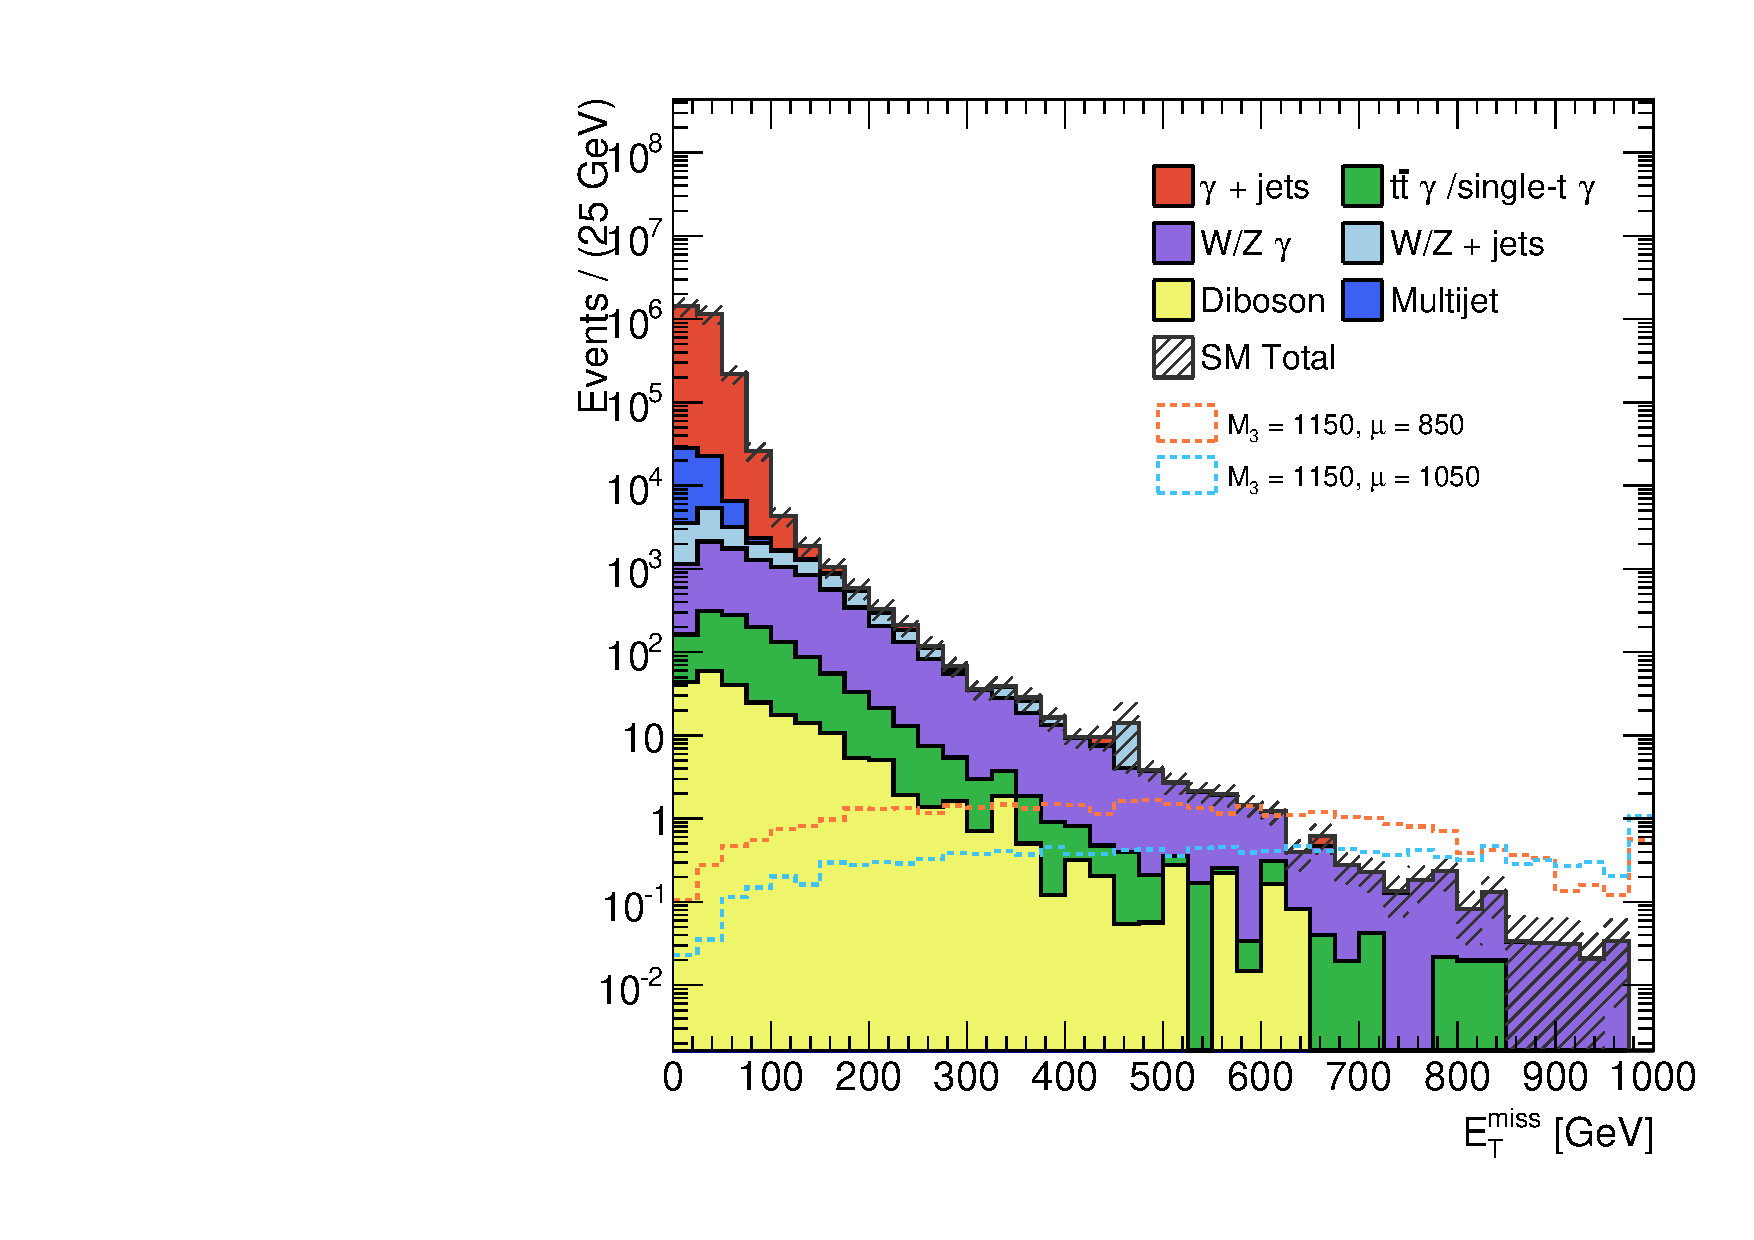
\includegraphics[width=0.49\textwidth]{met_et_base2}
  \caption{Energía faltante transversa
    luego de aplicar el corte en el {\pt} del fotón y en la energía de aislamiento
    para el fondo y los puntos de señal de {\SRL} (izquierda) y {\SRH} (derecha),
    para una luminosidad integrada de {\ilumi}.}

  \label{fig:opt_met}
\end{figure}



\subsection{Multiplicidad y {\pt} de los jets} \label{sec:opt_njet}

En la \cref{fig:jets_npv} se muestra el valor medio del número de jets
seleccionados como función del número de vértices en el evento, para distintos
cortes en el {\pt} de los jets. Notar que el número de vértices en un evento
está relacionado con el \emph{pile-up}. A medida que aumenta el corte en {\pt}
el número de jets se hace más estable con el \emph{pile-up}, y por lo tanto en
este análisis se consideran los jets con $\pt>40\gev$


\begin{figure}[!h]
  \centering
  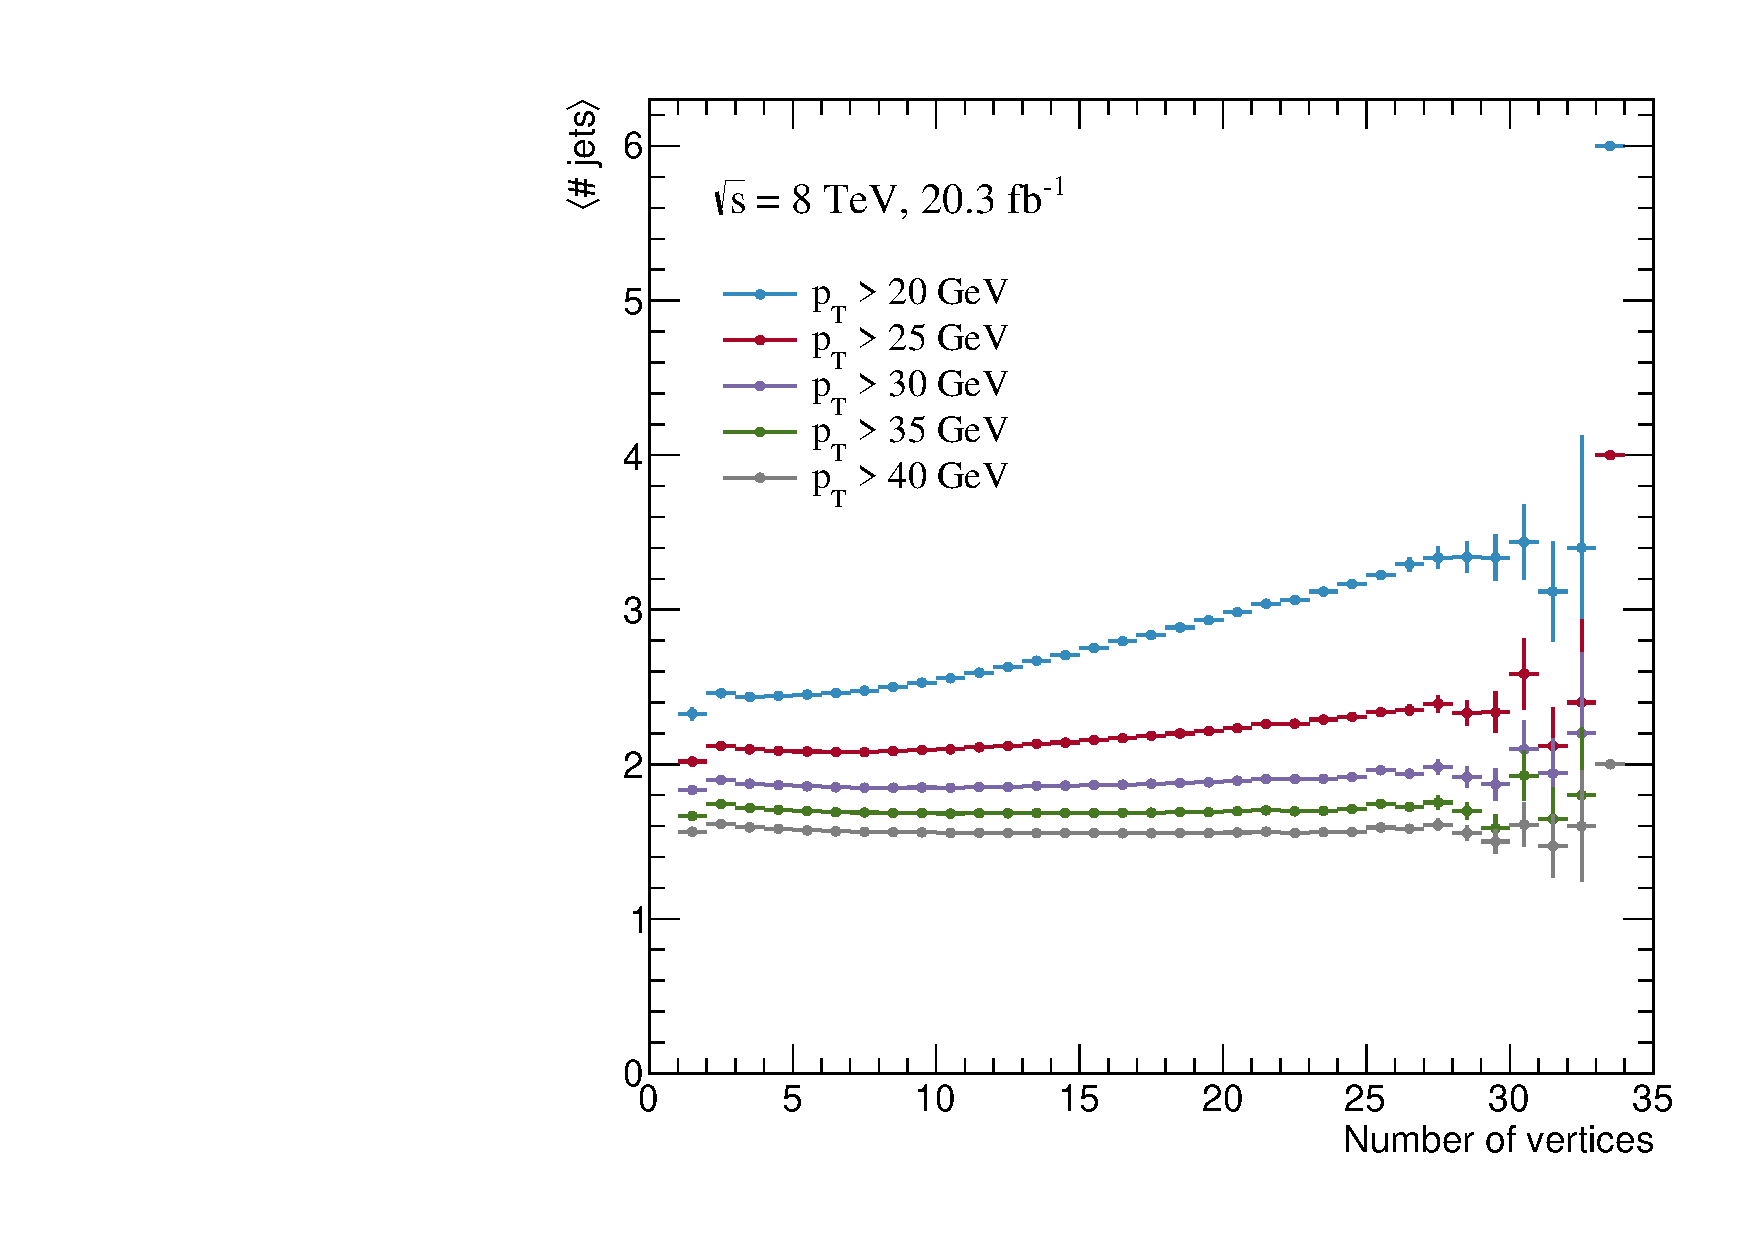
\includegraphics[width=0.5\textwidth]{data_jets_npv}
  \caption{Valor medio del número de jets vs. el número de vértices primarios
    observados en datos para distintas selecciones de $\pt^{\mathrm{jet}}$.}
    \label{fig:jets_npv}
\end{figure}


La \cref{fig:opt_jet_n} muestra la multiplicidad de jets (\njets)
para $\pt^{\mathrm{jet}} > 40$ \gev, después de los cortes optimizados en el
fotón y la {\met} descriptos anteriormente. Mientras que la señal tiene
típicamente un gran número de jets, la mayoría de los fondos W/Z+jets, diboson y
QCD se acumulan en la zona de pocos jets. Al menos dos (cuatro) jets son
requeridos para los eventos que pasan la selección de {\SRL} ({\SRH}). Una mayor
multiplicidad es efectivamente esperada para {\SRL} debido a que su objetivo es
la región de gluinos pesados donde el decaimiento dominante es el de producción
de charginos por un decaimiento de tres cuerpos.

\begin{figure}[!h]
  \centering
  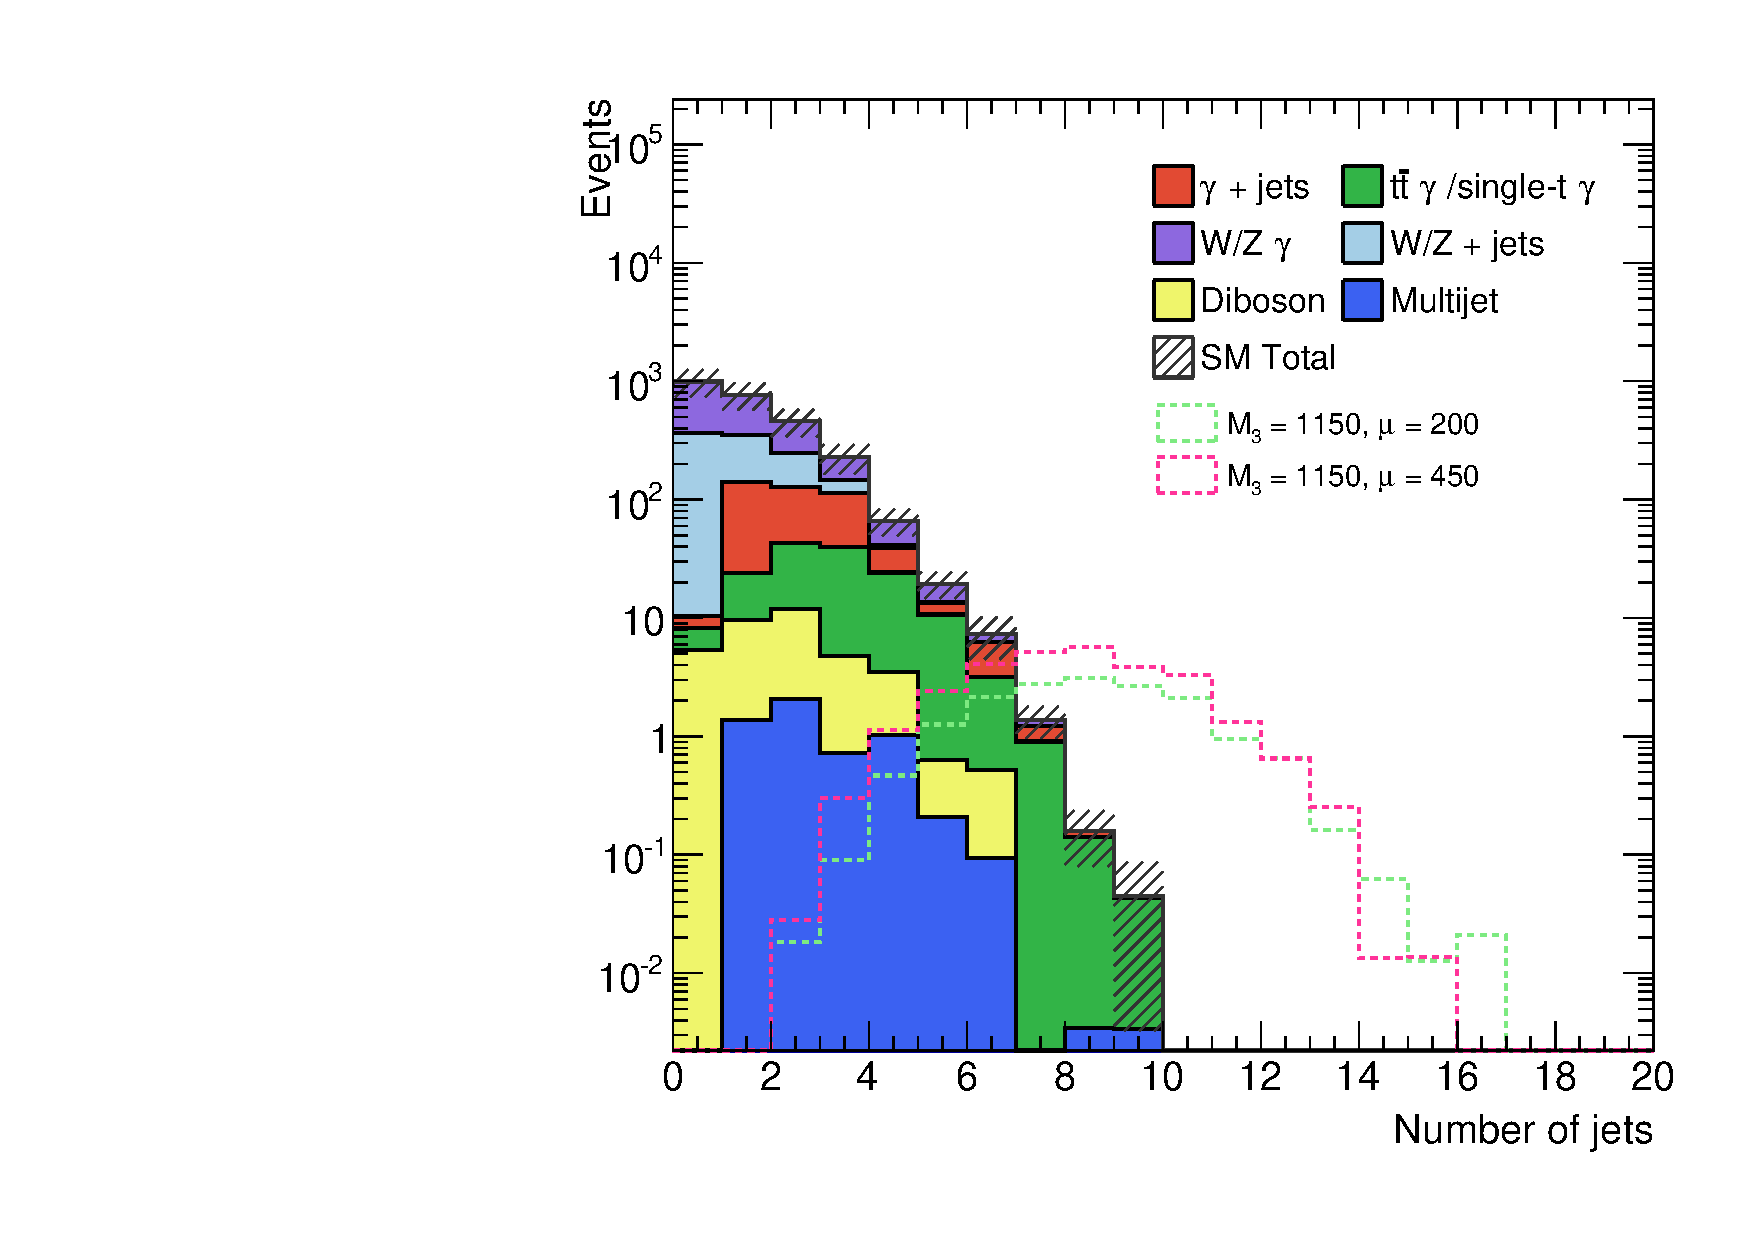
\includegraphics[width=0.49\textwidth]{jet_n_base1}
  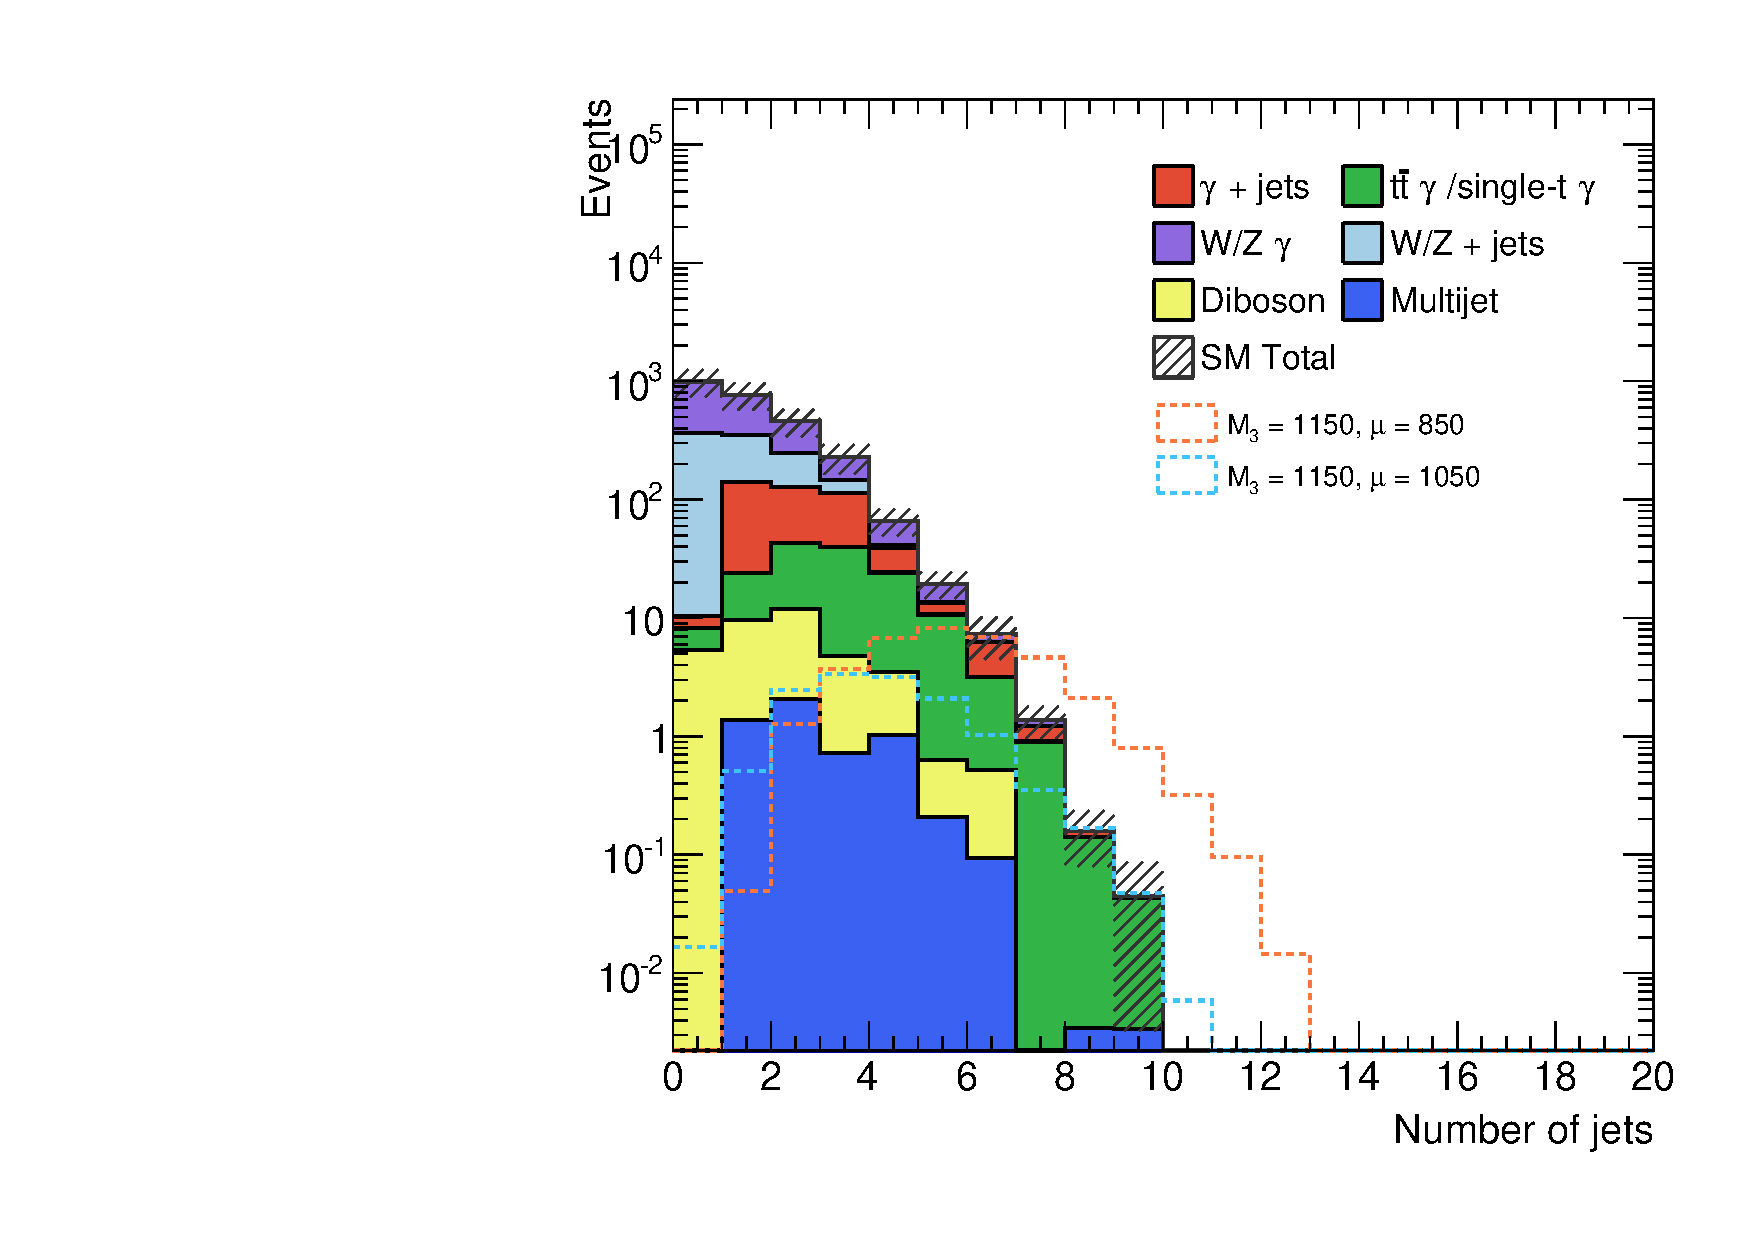
\includegraphics[width=0.49\textwidth]{jet_n_base2}
  \caption{Distribuciones del número de jets con $\pt > 40 \gev$ en {\SRL} (izquierda) y {\SRH} (derecha),
    después de la selección en el {\pt} del fotón y $\met > 150\gev$,
    para una luminosidad integrada de {\ilumi}.}
  \label{fig:opt_jet_n}
\end{figure}

%{\fig} \ref{fig:jetlead_3SR}  shows the \pt\ of the leading jet, after the photon \pt\ and \etmiss cut,
%and requiring the number of jets to be equal or larger than two for SR1-SR3, and equal or larger than
%four for SR2. Additional signal-background discrimination can be obtained by imposing cuts on the %leading
%jet \pt\ (\pt$(j1)$)since the signal tends to have hard leading jets, in particular for the case involving large
%gluino masses and low to medium neutralino masses (SR2).  For SR1 and SR2 the leading jet \pt\  is %required
%to be larger than 80 \gev~ and 100 \gev, respectively.   After those cuts, in  {\fig} \ref{fig:jetsublead_3SR},
%the subleading jet \pt\  (\pt$(j2)$) distributions for the three signal regions are shown. A further cut is %applied for
%SR1 and SR2, by requiring $\pt(j2)>80$ \gev~  and $> 100$ \gev, respectively.

%% La \cref{fig:opt_jet_p1} muestra el {\pt} del jet más energético ($\pt^{j1}$),
%% después de los cortes descriptos anteriormente. %Adicionalmenteafter the
%% photon \pt, \etmiss\ and $N_{jet}$ requirements described above for each signal region.

En la {\SRL} es posible obtener una discriminación requiriendo además que los dos jets
más energéticos tengan $\pt>100 \gev$.

%% En la {\SRH} donde la masa del gluino y la NLSP
%% es menor, een
%% Additional signal-background discrimination can be achieved by requiring a hard leading
%% jet, particularly for SR2 where the heavy gluinos decay down to relatively light neutralinos.
%% Thus, the leading jet \pt\ in SR2 is required to be larger than 100 \gev. Although a
%% harder requirement is suggested by {\fig} \ref{fig:jetlead_3SR}, it was found better to
%% keep it relatively loose and rely on the shape variables described in sec \ref{sec:shape_vars}.
%% The smaller mass difference between gluino and the lightest neutralino in SR3 leads to a
%% softer jet spectrum and then no further requirement is applied in this region.
%Additional signal-background discrimination can be obtained by imposing cuts on the leading  jet \pt\ since the signal tends to have hard leading jets, in particular for the case involving  large gluino masses and low to medium neutralino masses (SR2).  For SR1 and SR2 the leading jet \pt\  is required to be larger than 80 \gev~ and 100 \gev, respectively.

%% \begin{figure}[!htbp]
%%   \centering
%%   \includegraphics[width=0.49\textwidth]{figures/figura} %jet1_pt_SR2}
%%   \includegraphics[width=0.49\textwidth]{figures/figura} %jet1_pt_SR3}
%%   \caption{Momento transverso del jet más energético en {\SRL} (izquierda) y {\SRH} (derecha),
%%     para una luminosidad integrada de {\ilumi}.}
%%   \label{fig:opt_jet_pt1}
%% \end{figure}

%% A continuacion se exploro el momento transverso del segundo jet más energetico ($\pt^{j2}$).
%% Las distirbuciones para cada region pueden verse en \cref{fig:opt_jet_pt2}. En {\SRL}
%% se encontro que un corte en $\pt^{j2}>100$ \gev

%% \begin{figure}[!htbp]
%%  \centering
%%  \includegraphics[width=0.49\textwidth]{figures/figura} %jet2_pt_SR2}
%%  \includegraphics[width=0.49\textwidth]{figures/figura} %jet2_pt_SR3}
%%   \caption{Momento transverso del segundo jet más energético en {\SRL} (izquierda) y {\SRH} (derecha),
%%     para una luminosidad integrada de {\ilumi}.}
%%  \label{fig:opt_jet_pt2}
%% \end{figure}



\subsection{Separación angular entre jets y \met}
\label{sec:dphi_obj}

Como ya ha sido mencionado, en los eventos de señal, la energía faltante es producida por los dos
gravitinos que escapan la detección. Se espera por lo tanto que la dirección de {\met} sea aleatoria,
sin estar correlacionada con ninguno de los demás objetos del evento. Por otro
lado, si la {\met} es originada a partir de efectos instrumentales o de neutrinos
energéticos en $b$-jets o $c$-jets, la dirección de {\met} estará
correlacionada con uno de los jets mal reconstruidos. La
\cref{fig:opt_dphi_jetmet} muestra el mínimo $\Delta\phi$ entre la dirección
de {\met} y la de los dos jets más energéticos.

%% \begin{equation} \label{eq:dphi}
%%   %%\min\left[ \cos   \Delta\phi({\rm jet}_{1,2},\MET) \right] \equiv  \min \left[\frac{\vec{\met} \cdot \vec{p}_{\rm T}^{\rm \; jet,i}}{|\vec{\met}|  |\pt^{\mathrm{jet},i}|}\right] \quad \quad i = 1,2
%%   \cos \Delta\phi(\mathrm{jet},\met) \equiv \frac{\vec{\met} \cdot \vec{p}_\mathrm{T}^{\mathrm{jet}}}{|\vec{\met}| |\pt^{\mathrm{jet}}|}
%% \end{equation}
%% %

%% after applying the photon \pt, \met, jet {\pt} and multiplicity cuts.
%% A lower bound $\dphijm>0.4$ cut is applied for the two signal regions,
%% which helps to significantly reduce the QCD background and clean events with mis-reconstructed \etmiss.

\begin{figure}[!h]
  \centering

  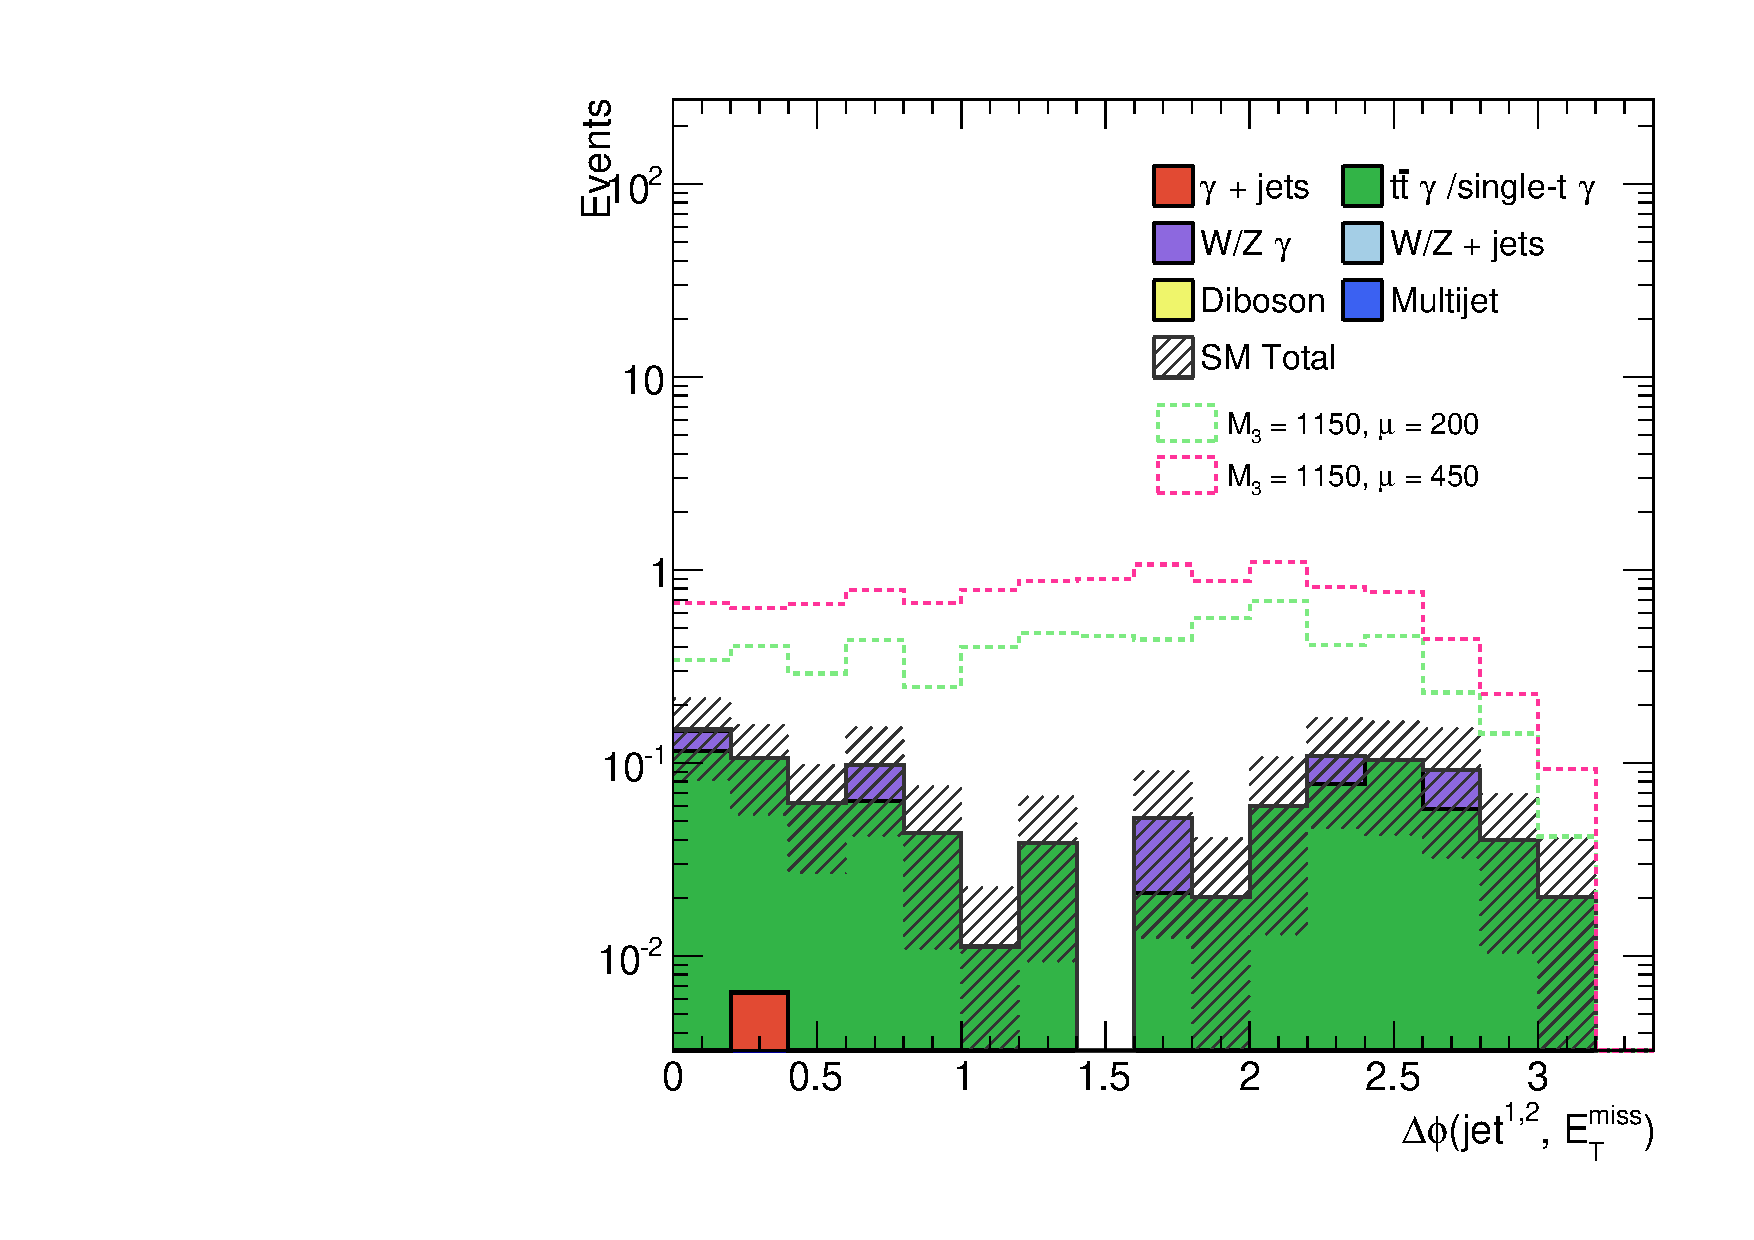
\includegraphics[width=0.49\textwidth]{figures/dphi_jetmet_srl}
  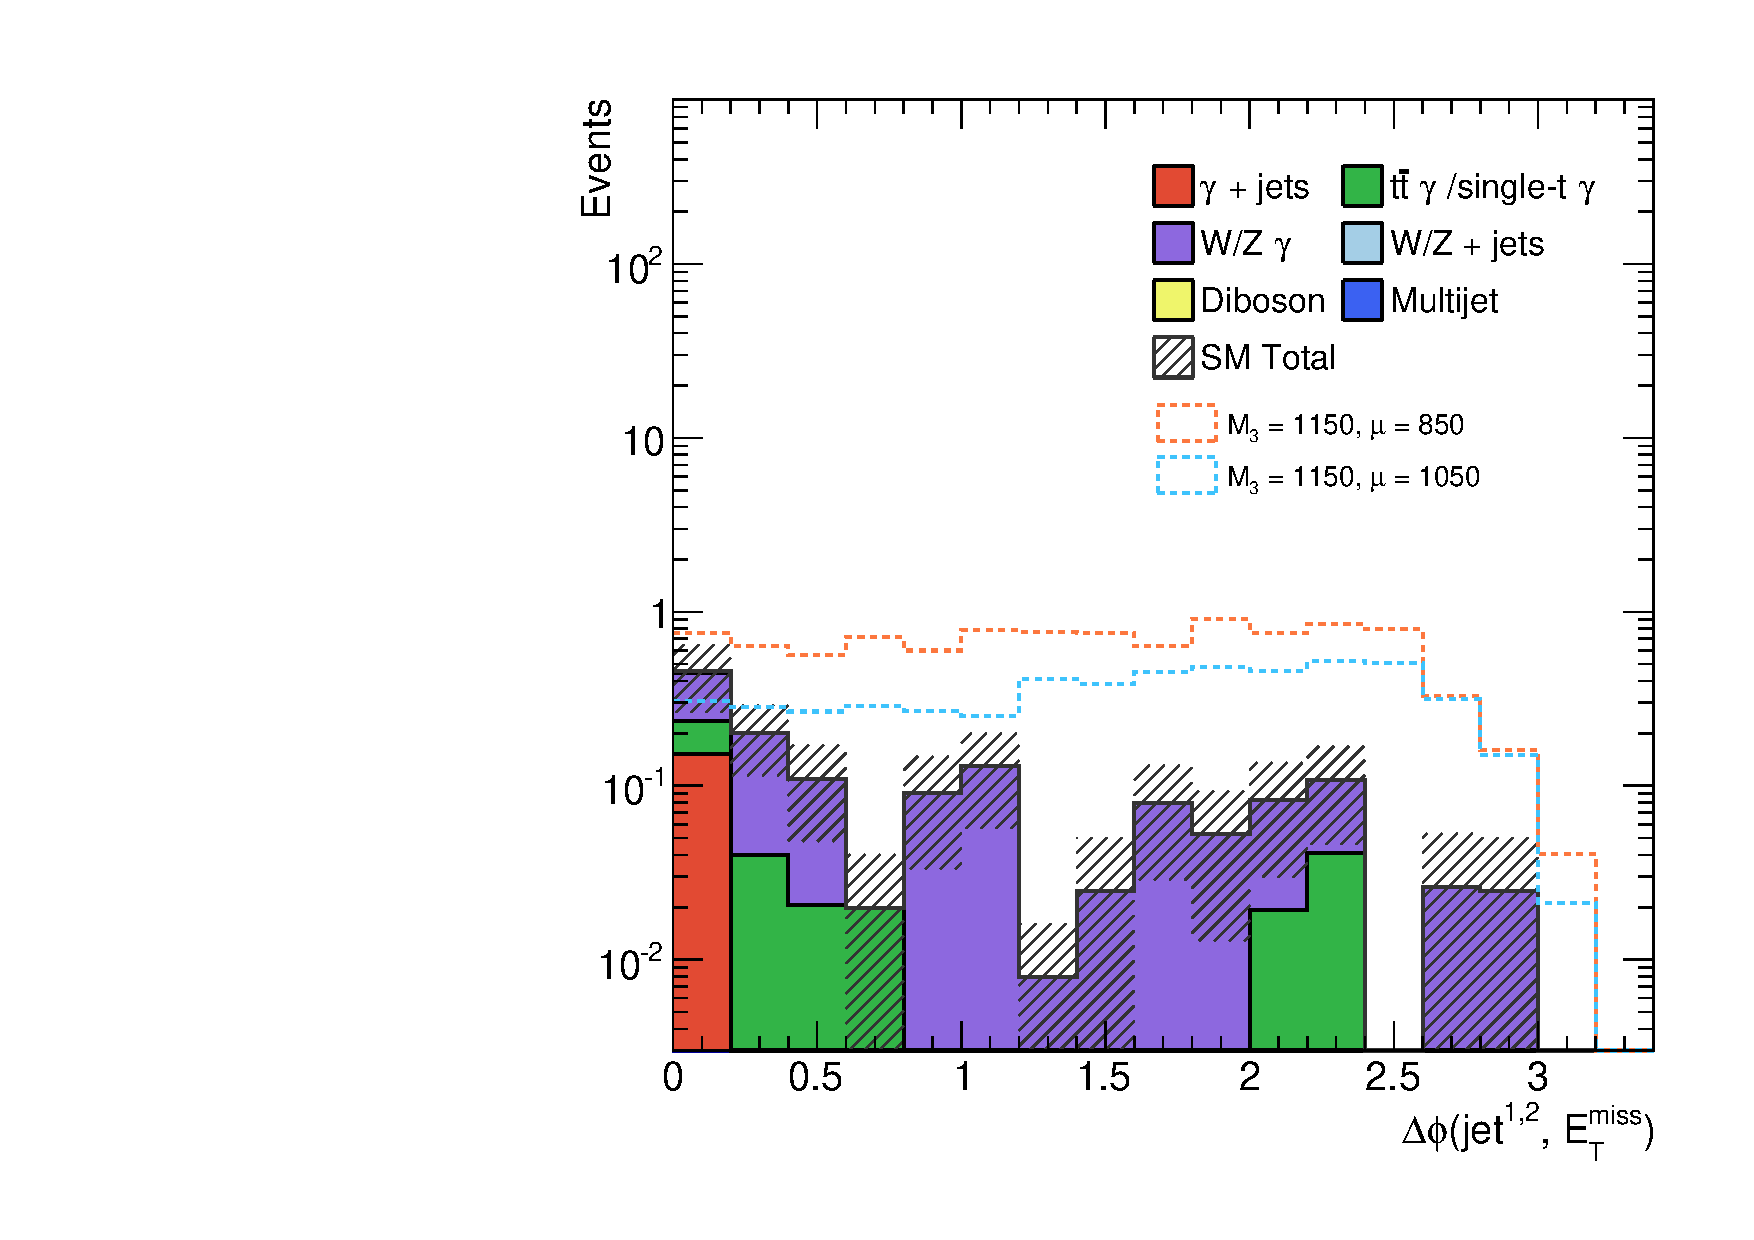
\includegraphics[width=0.49\textwidth]{figures/dphi_jetmet_srh}

  \caption{Separación angular $\Delta \phi \mathrm{(jet, \met)}$ para el fondo y los puntos de se\~nal para {\SRL} (izquierda) y {\SRH} (derecha),
    para una luminosidad integrada de {\ilumi}.}
  \label{fig:opt_dphi_jetmet}
\end{figure}


\subsection{Separación angular entre jets y fotón}

Para regiones del espacio de parámetros del modelo de señal
donde los gluinos y los neutralinos tienen alta masa ({\SRH})
un corte en la separación entre el fotón y los jets ayuda a
reducir el fondo, principalmente aquel proveniente de dijets y
fotones directos, donde un fotón (real o falso) tiende a ser
producido en la dirección opuesta al jet más energético.
La distribución para la {\SRH} se puede ver en \cref{fig:opt_dphi_gamjet}.


\begin{figure}[!h]
  \centering

  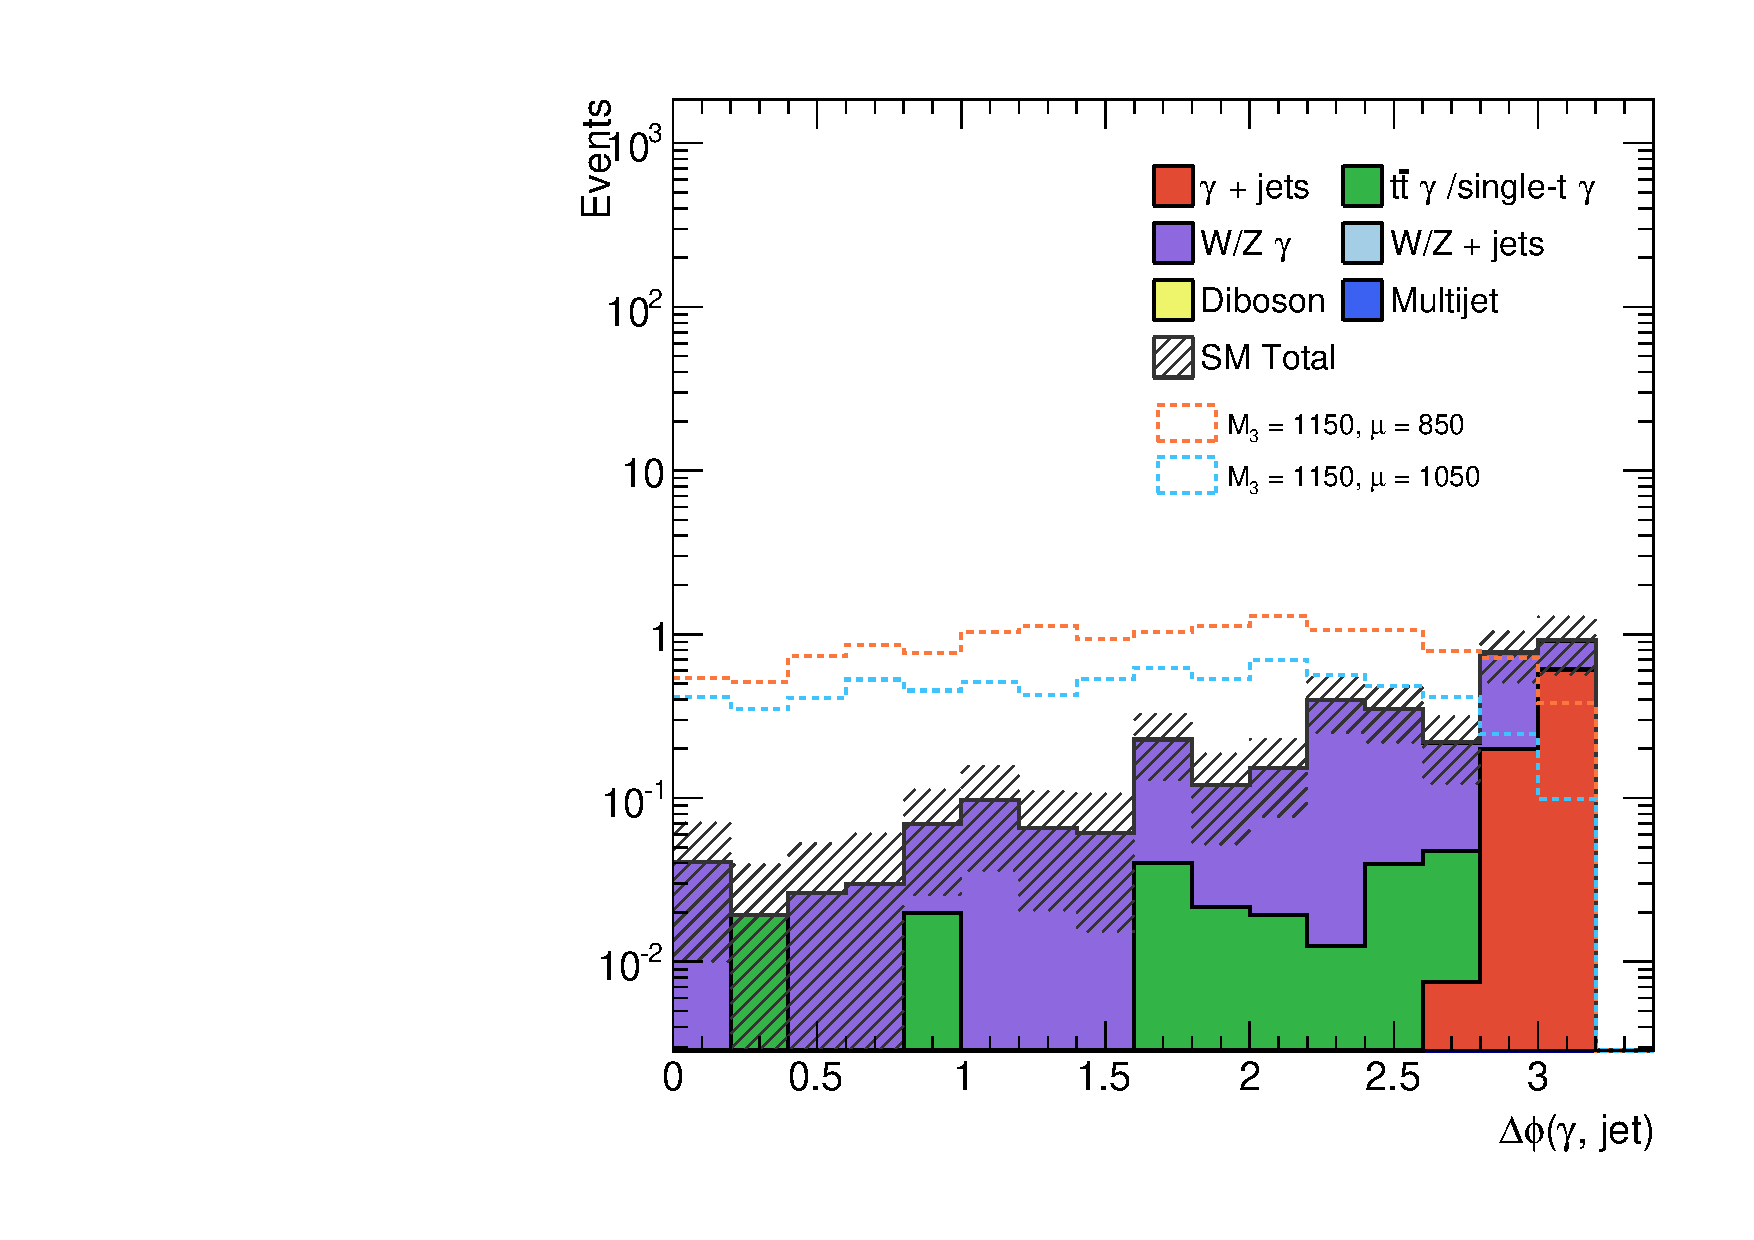
\includegraphics[width=0.49\textwidth]{figures/dphi_gamjet_srh}

  \caption{Distribución de {\dphijg} para {\SRH}, después de aplicar la selección completa, excepto este corte,
    para una luminosidad integrada de 20.3 \ifb.}
  \label{fig:opt_dphi_gamjet}
\end{figure}



\subsection{Energía total transversa (\HT)}
\label{sec:ht_obj}

Dada la gran masa de los gluinos producidos en las colisiones, en el espacio de
parámetros explorado en este análisis, se espera que la energía transversa
visible total sea alta. Por eso, el observable {\HT} definido como la suma
escalar del momento transverso de todos los objetos observados en el estado
final es mucho mayor para eventos de señal que para los eventos de fondo.
Después del veto a los eventos con leptones, {\HT} se define como:

\begin{equation}
  \HT \equiv |\pt^{\gamma}| + \sum_{\mathrm{jets}} |\pt^\mathrm{jet}|
  \label{eq:ht_def}
\end{equation}

La \cref{fig:opt_ht} muestra las distribuciones de {\HT} para las dos regiones de señal.
Para {\SRL}, se espera incluso que {\HT} sea mayor, debido a la
diferencia de masa entre el gluino y el neutralino NLSP. Sin embargo
se encontró una variable más efectiva para la separación entre señal y
fondo que se describe a continuación y por lo tanto no se aplica un corte
en esta variable.

En {\SRH} un corte en este observable $\HT>800\gev$ ayuda a reducir el fondo restante.
Dada la masa alta del neutralino, la mayor contribución de {\HT} proviene
del fotón muy energético producido en el evento.


\begin{figure}[!h]
  \centering

  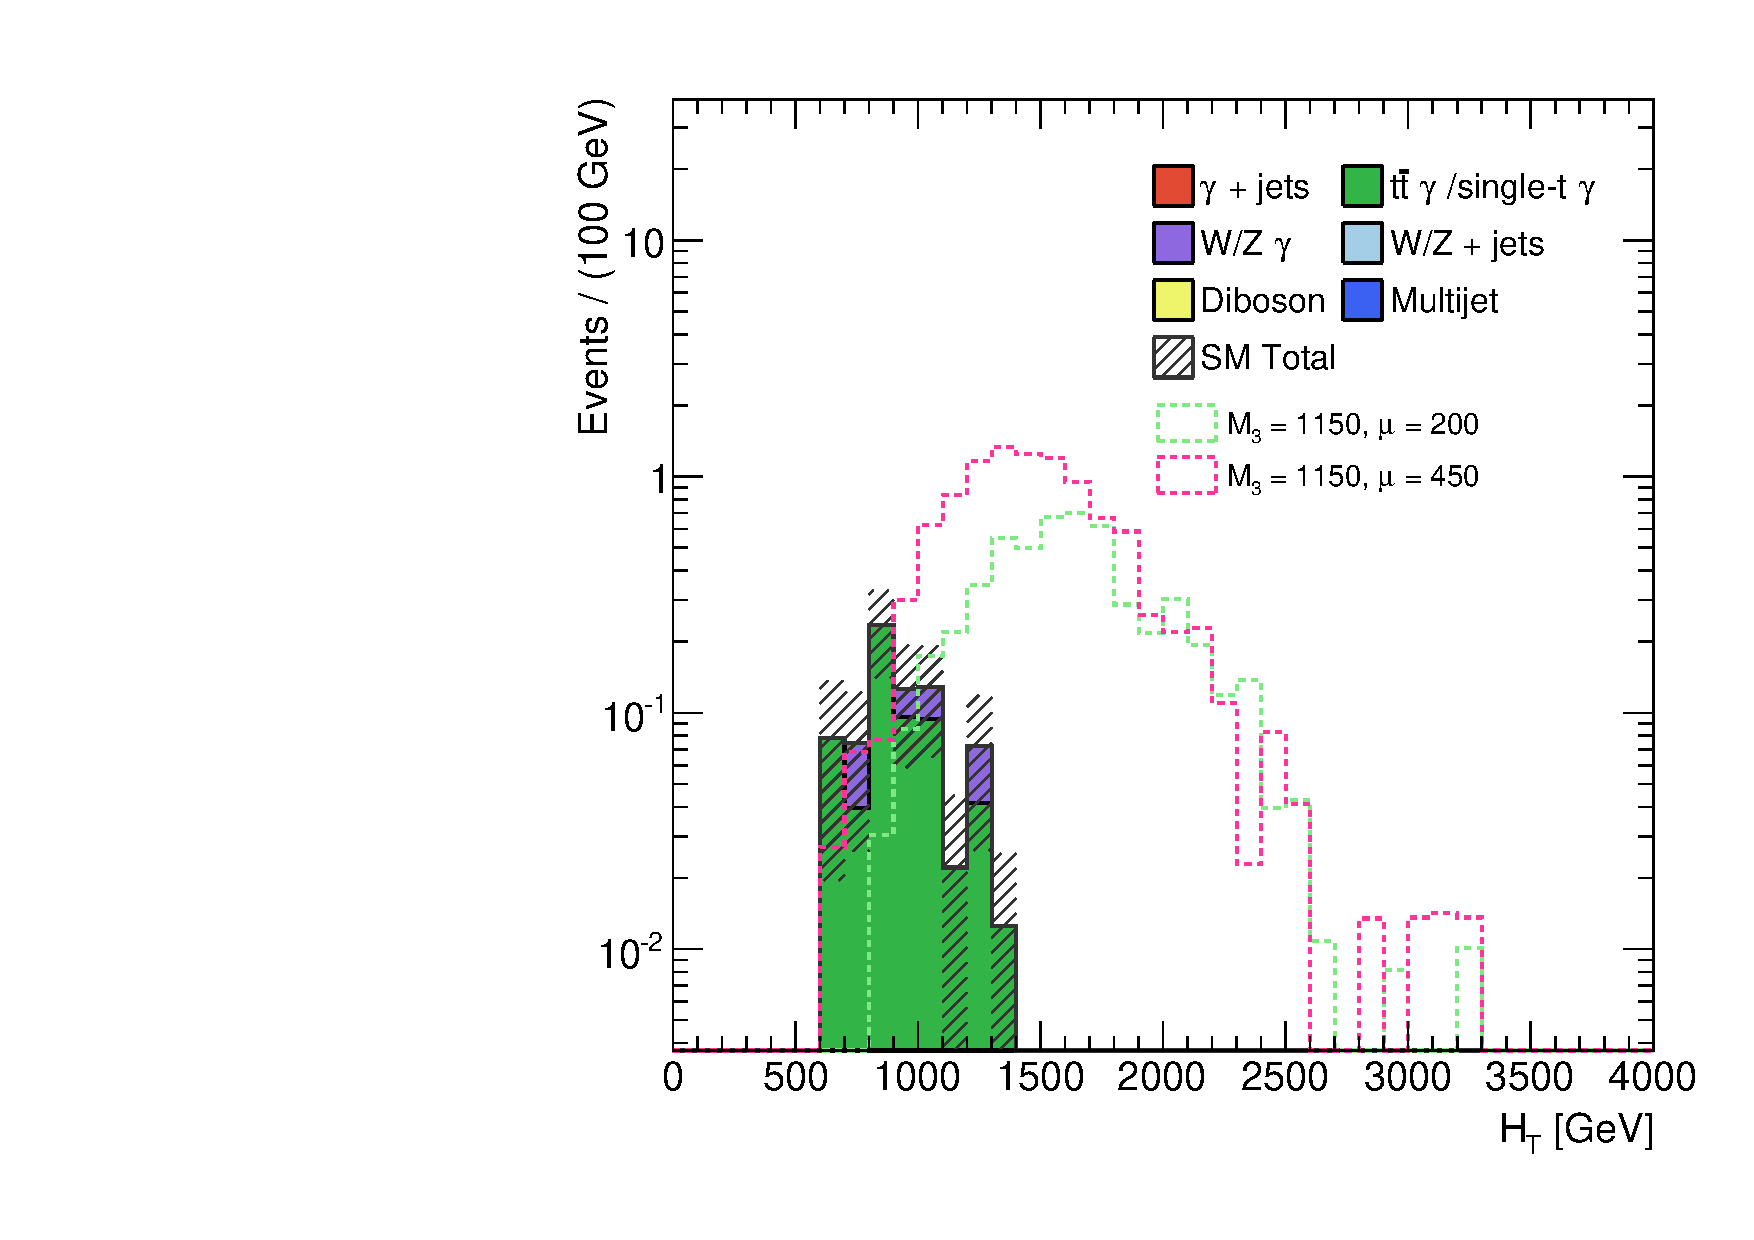
\includegraphics[width=0.49\textwidth]{ht_srl}
  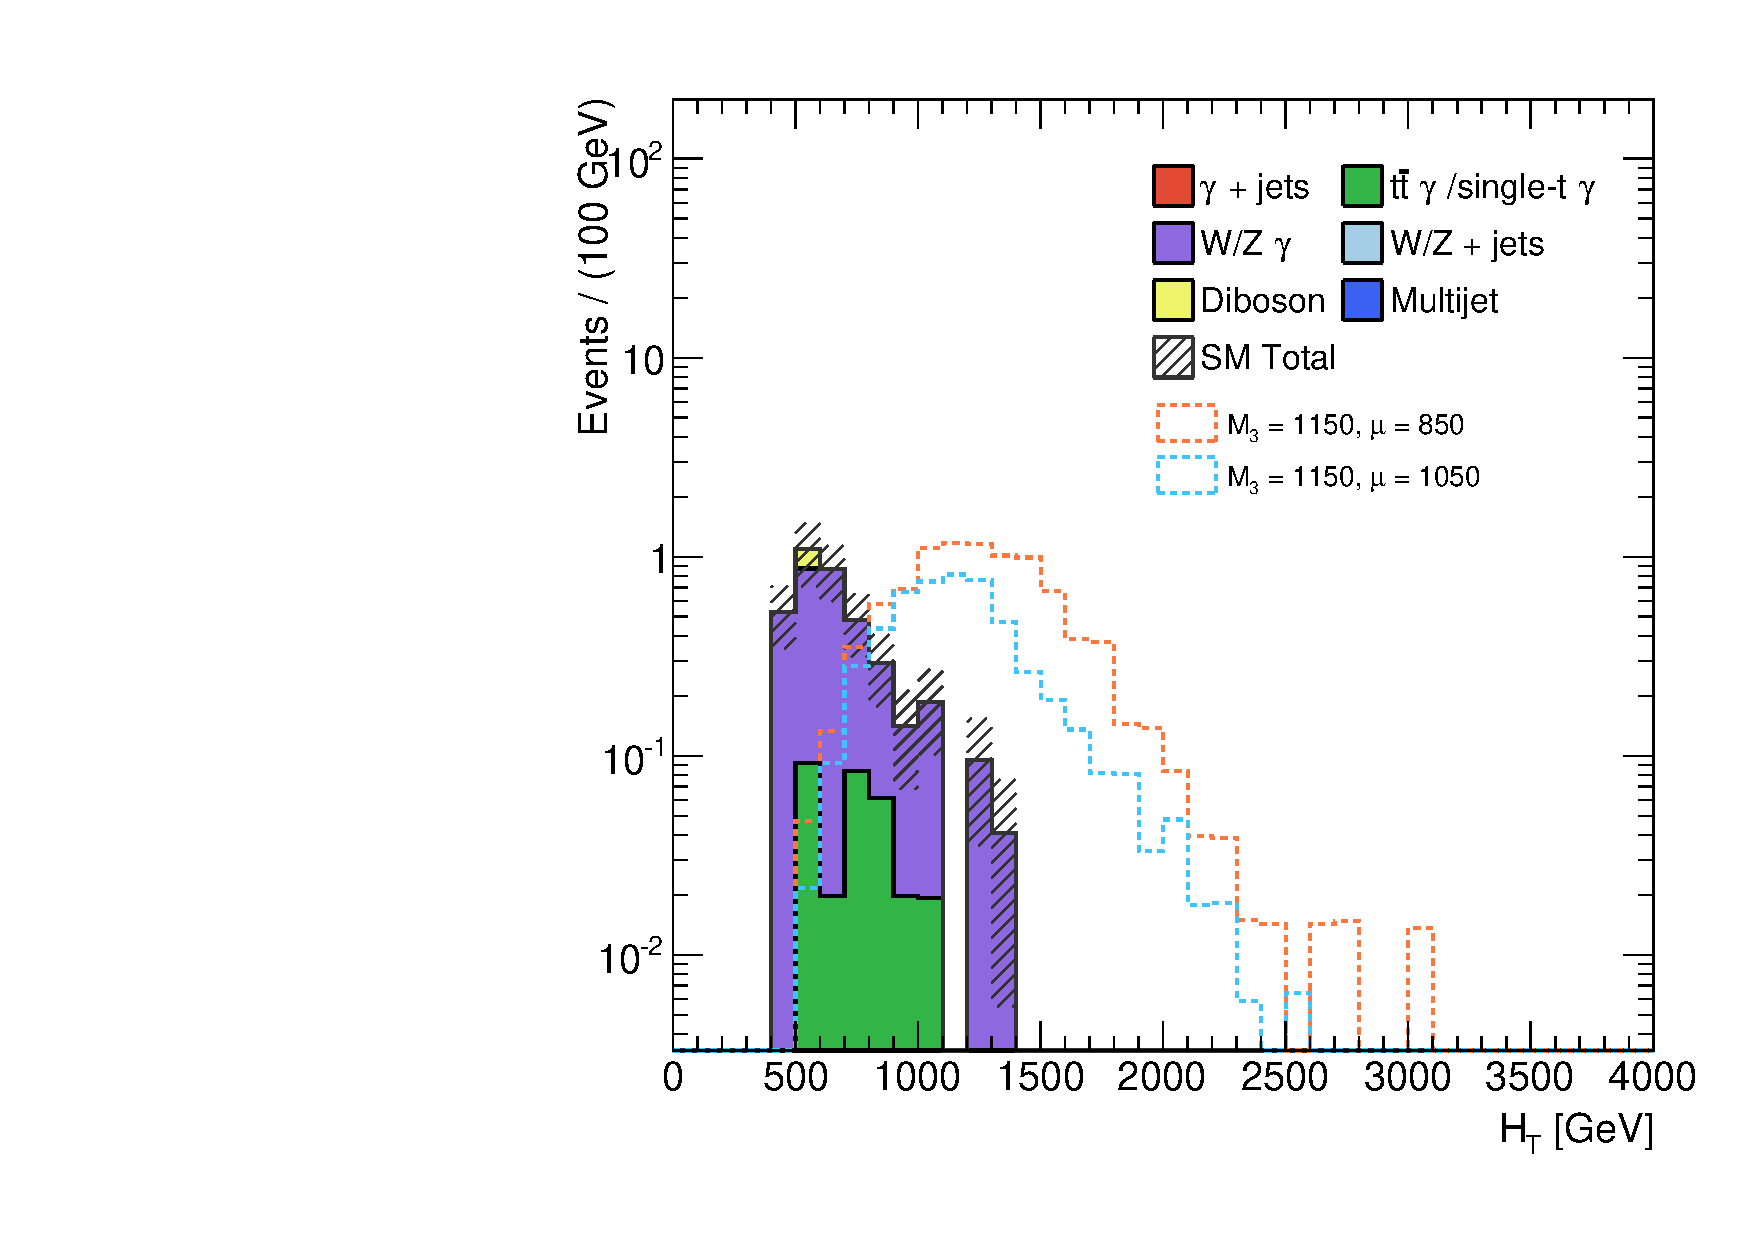
\includegraphics[width=0.49\textwidth]{ht_srh}

  \caption{Distribución de la energía total transversa (\HT) para {\SRL} (izquierda)
    y {\SRH} (derecha) para una luminosidad total integrada de 20.3 \ifb. Todos los cortes de la selección
  de la SR son aplicados exceptuando el corte en {\HT}.}
  \label{fig:opt_ht}
\end{figure}



\subsection{Variables de forma adicionales}\label{sec:shape_vars}

Varias variables de forma fueron exploradas para poder obtener
una discriminación adicional entre señal y fondo. En especial se estudió el
observable $R_T^n$ definido como

\begin{equation}\label{eq:rt_formula}
  R_\mathrm{T}^{n} = \frac{\sum_{i=1}^{n}p_\mathrm{T}^{\text{jet}_i}}{\sum p_\mathrm{T}^{\text{jet}}},
\end{equation}
%
es decir, el cociente entre la suma escalar de los {\pt} de $n$ jets y la suma
escalar del {\pt} de todos los jets en el evento, donde $n$ es el mínimo número
de jets requerido.

Es evidente que la distribución de esta variable (como se explica en
\cite{PhysRevD.84.055010}), depende de la multiplicidad y el momento transverso
de los jets. En el caso que $n \sim \njets$ el denominador y el
numerador son casi idénticos y el cociente es $\sim 1$, y es exactamente 1
cuando son iguales.
Para los procesos de señal en los que $n$ es mucho menor al número de jets en el
evento, la distribución será menor a 1.


\begin{figure}[!h]
  \centering

  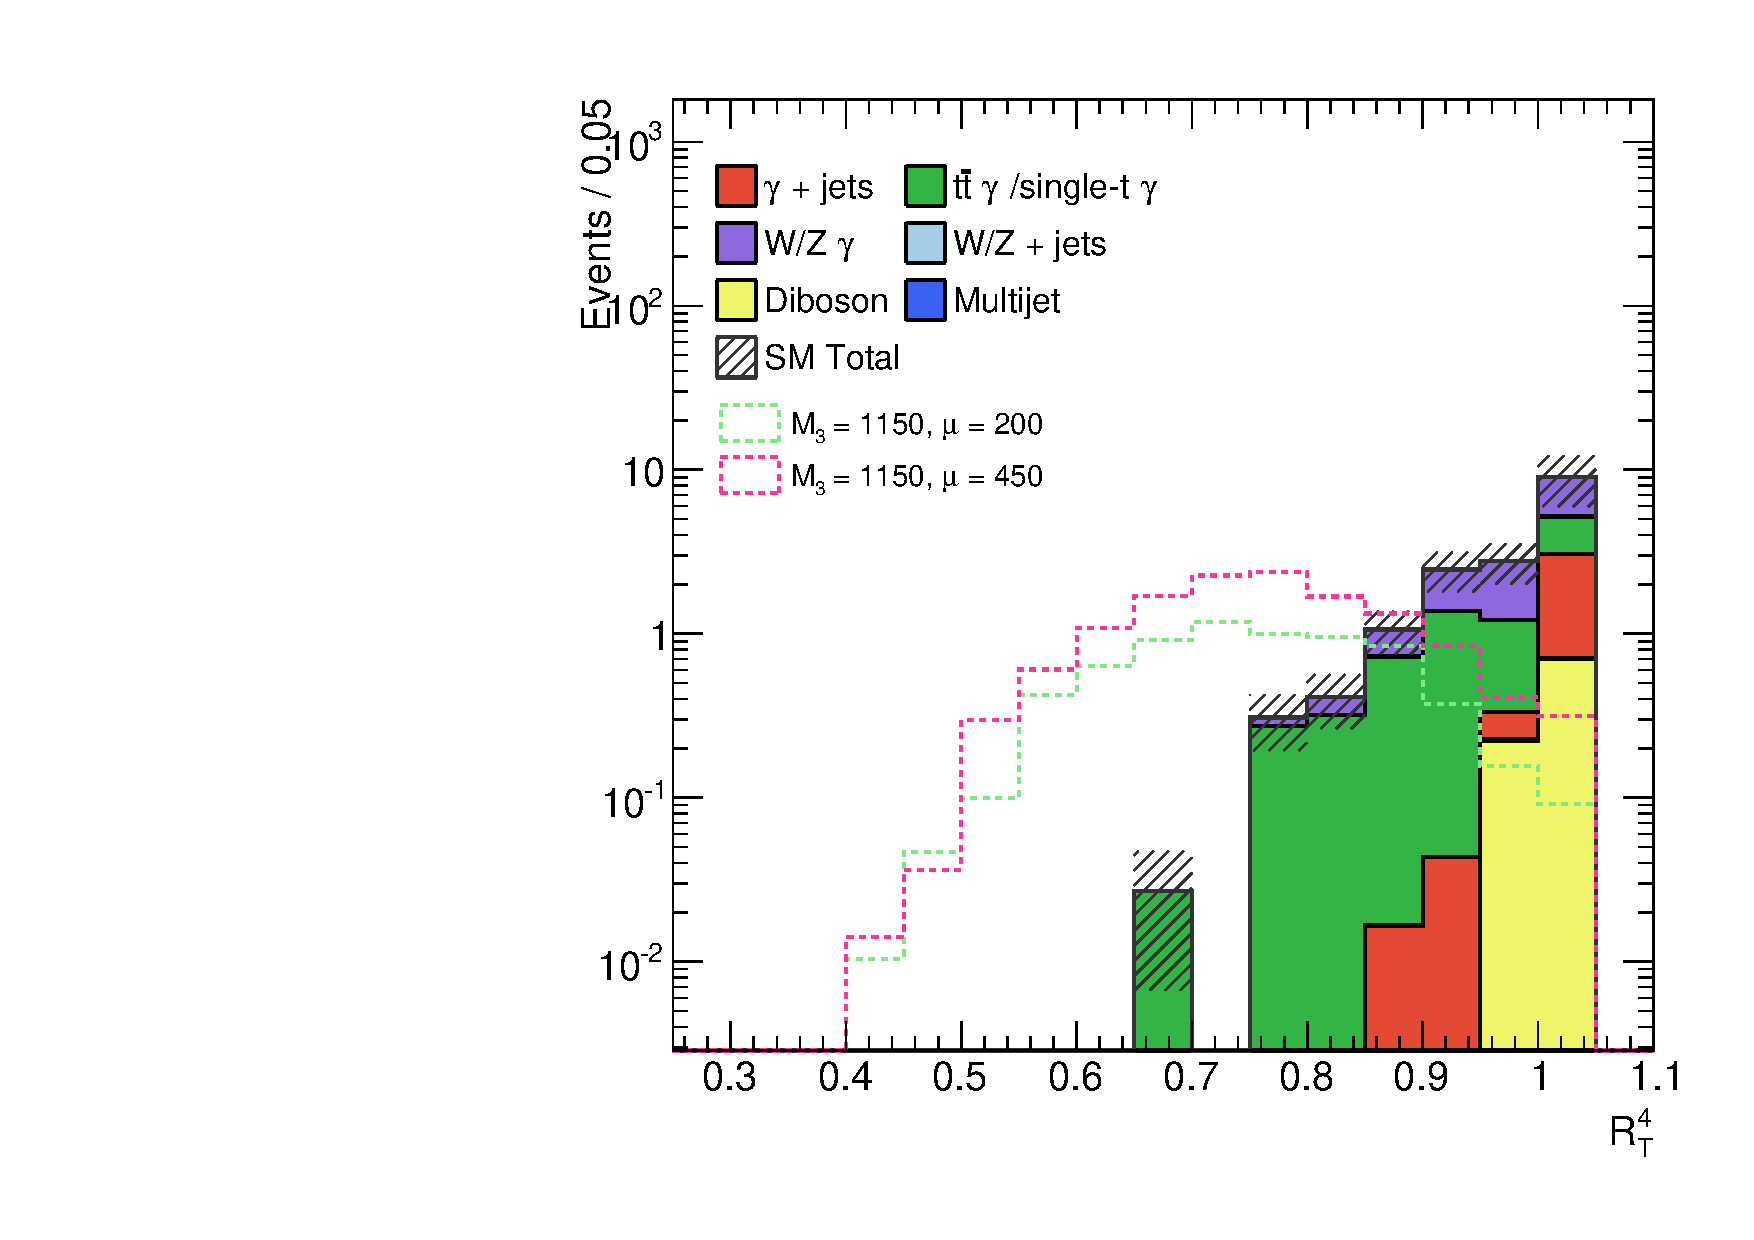
\includegraphics[width=0.49\textwidth]{figures/rt4_srl}
  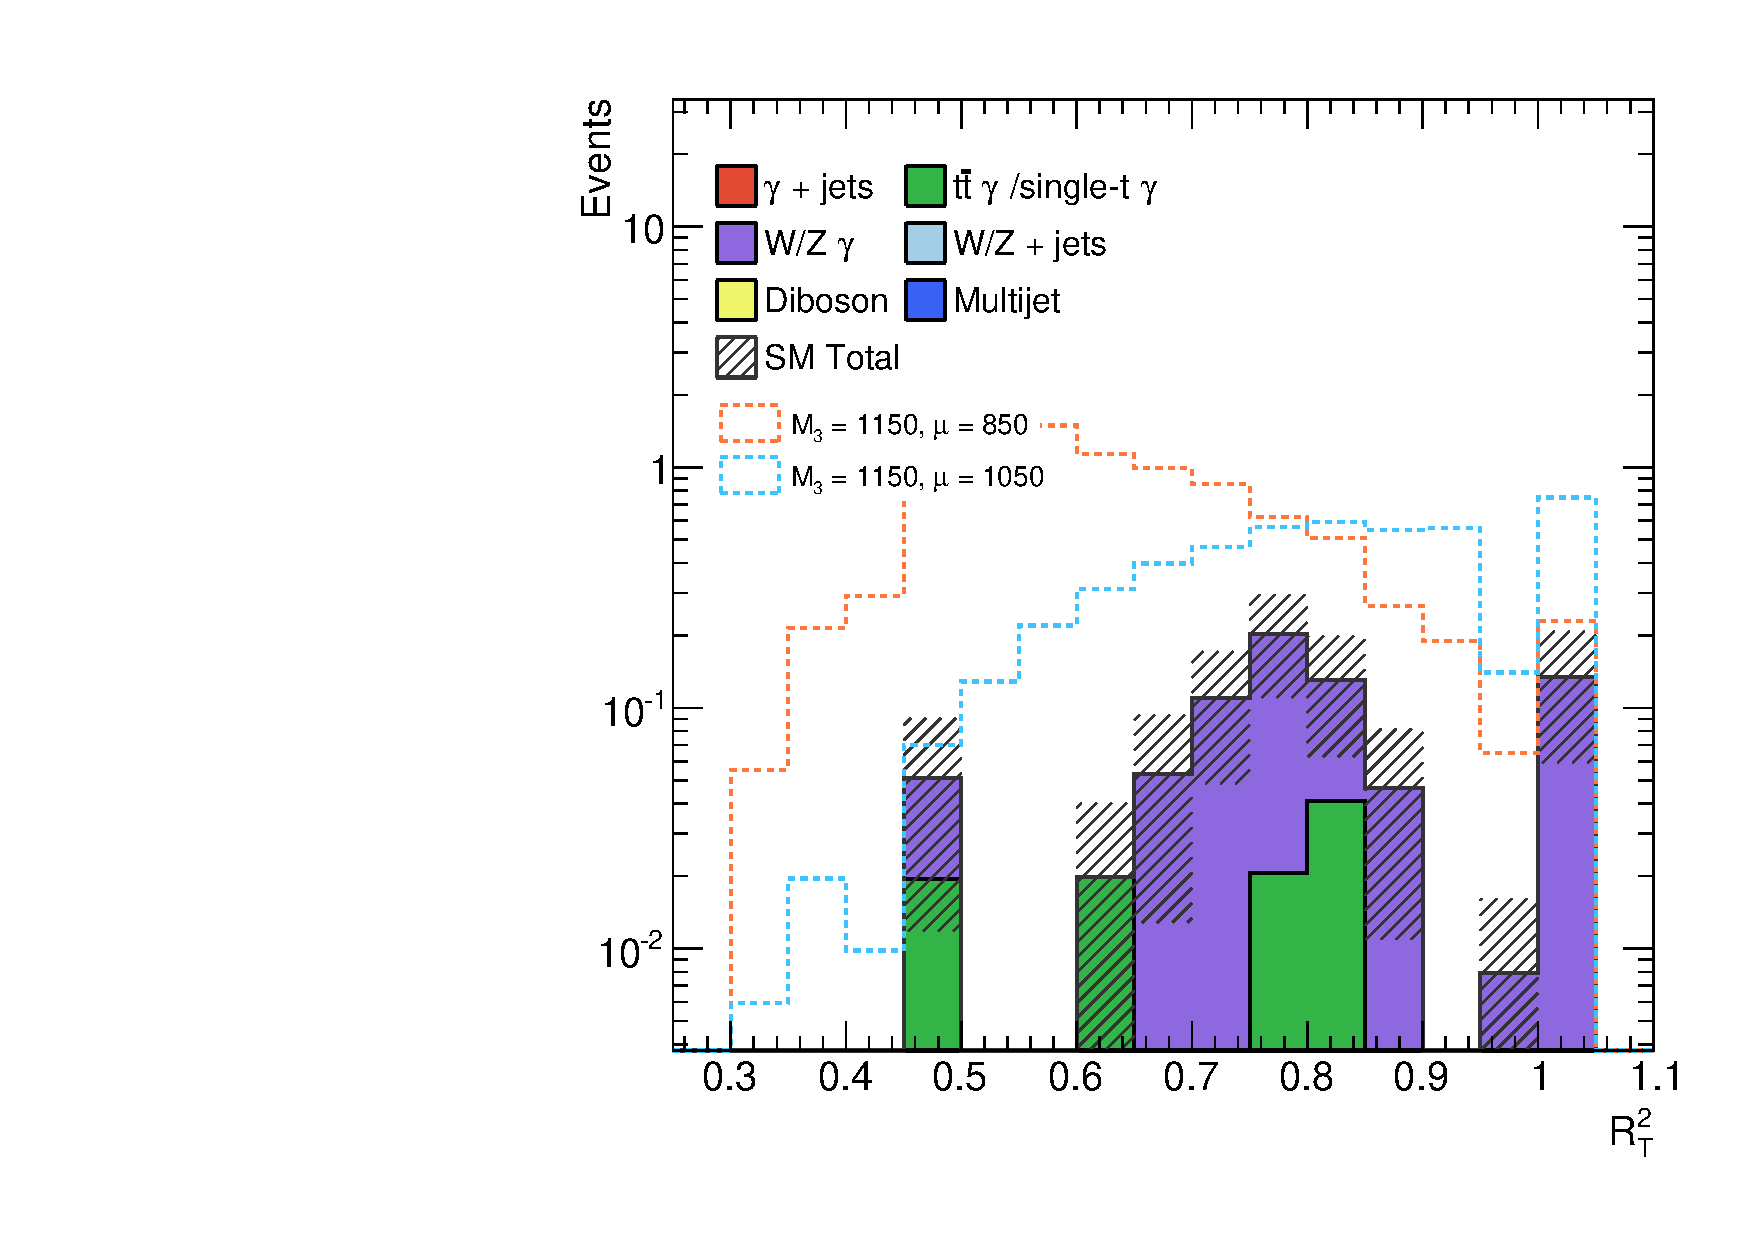
\includegraphics[width=0.49\textwidth]{figures/rt2_srh}

  \caption{Distribución de {\rt} para {\SRL}  (izquierda) y {\rtt} para {\SRH} (derecha)
    para una luminosidad total integrada de 20.3 \ifb. Todos los cortes de la selección
    de la SR son aplicados exceptuando el corte en $R_\mathrm{T}$.}
  \label{fig:opt_rt}
\end{figure}

La \cref{fig:opt_rt} (izquierda) muestra la distribución de {\rtt} para {\SRH},
después de la selección final excepto el corte en {\rtt}. Mientras que la
\cref{fig:opt_rt} muestra la distribución de {\rt} para {\SRL}. El bajo número
de jets para {\SRH}, hace que la distribución de {\rtt} para los eventos de
señal sea similar a la del fondo QCD, y por lo tanto el observable no es útil
para rechazar fondo manteniendo una aceptancia razonable. Para el caso de {\SRL}
un corte $\rt < 0.85$ permite reducir en una fracción considerable el fondo con
una pérdida muy chica en la eficiencia de señal.



\section{Selección final de las regiones de se\~nal}\label{sec:signal_regions}

Como resultado del proceso de optimización descripto en la sección anterior,
se definen las dos regiones de señal:

\begin{description}\itemsep0.2cm

\item[{\bf {\SRL}}] motivada por los eventos en los que gluinos
  decaen a neutralinos de baja/media masa. Estos eventos están
  caracterizados por una gran multiplicidad de jets energéticos, mientras que la energía
  del fotón y la energía faltante dependerá de la masa del neutralino, pero en general
  será relativamente baja.


\item[{\bf {\SRH}}] motivada por eventos en los que los gluinos
  producidos decaen en neutralinos con una masa similar a estos. Dichos eventos están caracterizados
  por un fotón de alto {\pt} y gran cantidad de {\met}, con una menor multiplicidad de jets.
\end{description}

Cada región de señal queda definida entonces por los cortes de selección detallados en la \cref{tab:final_sel_sr}.

\begin{table}[!htbp]

  \centering
  \caption{Conjunto de cortes en los observables que definen las dos regiones de señal, {\SRL} y {\SRH}.}
  \label{tab:final_sel_sr}

  \begin{tabularx}{0.6\textwidth}{LRR}
    \hline
    & {\SRL} & {\SRH} \\
    \hline
    {\nphotons} & $=1$ & $=1$ \\
    \ptgam & $>125 \gev$ & $>300 \gev$ \\
    {\nleptons} & $=0$ & $=0$ \\
    {\njets} & $\geq 4$ & $\geq 2$ \\
    $\pt^{\mathrm{jet}_1}$ & $>100 \gev$ & - \\
    $\pt^{\mathrm{jet}_2}$ & $>100 \gev$ & - \\
    $\Delta\phi(\mathrm{jet}, \met)$ & $>0.4$ & $>0.4$ \\
    {\met} & $>200 \gev$ & $> 300 \gev$ \\
    $R_\mathrm{T}^4$ & 0.85 & - \\
    $\HT$ & - & $>800 \gev$ \\
    $\Delta\phi(\gam,\mathrm{jet})$ & - & $<2.0$ \\
    \hline
    \end{tabularx}

\end{table}


El número esperado de eventos de fondos del {\SM} estimado a partir de de las
muestras simuladas después de la selección final se muestra en la
\cref{tab:exp_bkg_sr}, para {\SRL} y {\SRH},
respectivamente. También se presenta el número de eventos esperado de señal y la
significancia esperada para los dos puntos de referencia en cada SR.
Adicionalmente, en la \cref{tab:mc_events_sr_phtype} se puede ver el número de
eventos de fondo esperado separando fotones reales de los eventos donde un jet o
un electrón es identificado erróneamente como un fotón.
%% El primer tipo de eventos es claramente
%% dominante en este análisis, en presencia de energía faltante tanto real como
%% instrumental.
Se puede ver que la contaminación dominante proviene de {\vgam} ($V=W \text{ o }
Z$) y {\ttgam}. La contaminación de {\vgam} en {\SRL} es de 0.13, de los cuales
0.10 corresponden a {\wgam} y 0.03 a {\znngam}. Para {\SRH} el número de eventos
de {\vgam} es de 0.66, de los cuales 0.44 de {\wgam} y 0.22 de {\znngam}. En la
{\SRL} también existe una contaminación de eventos de procesos {\ttbar} en los
que un electrón es identificado como fotón.

La significancia esperada de descubrimiento para los distintos puntos
de la \emph{grid} de señal en el plano {\mgmn} se puede ver en la
\cref{fig:opt_discovery_exp}, junto con los contornos en los que la significancia
es de $3\sigma$ y $5\sigma$.

Es
importante notar que estos resultados son preliminares y obtenidos de
simulaciones Monte Carlo. Los resultados finales son derivados utilizando los
métodos de estimación de fondos descriptos en el \cref{cap:fondos}, y luego
del ajuste combinado, y son descriptos en el \cref{cap:resultados}.

\begin{table}[!h]
  \centering
  \caption{Número de eventos esperado para los fondos del {\SM}
    y algunos puntos de señal después de cada corte de la región
    de señal {\SRL} (arriba) y {\SRH} (abajo), para una luminosidad integrada de {\ilumi}. Para los
    puntos de señal, también se muestra en la última fila, la
    significancia esperada.}

  \label{tab:exp_bkg_sr}

  \resizebox{\textwidth}{!}{
    \begin{tabular}{lrrrrrrrrr}
      \hline
      \multicolumn{1}{c}{\textbf{\SRL}}   & \multicolumn{1}{c}{(1150, 200)} & \multicolumn{1}{c}{(1150,450)} &  \multicolumn{1}{c}{V\gam} & \multicolumn{1}{c}{Diboson} & \multicolumn{1}{c}{V + jets} & \multicolumn{1}{c}{\gjet, multijet} & \multicolumn{1}{c}{\ttbar} & \multicolumn{1}{c}{\ttgam} & \multicolumn{1}{c}{Fondo total} \\
      \hline
      $=1$ fotón        &  22.87 & 33.75 & 8396.04 & 230.19 & 10093.10 & 3103339.25 & 251.46 & 847.09 & $3123157.13\pm2013.86$ \\
      0 leptones        &  13.66 & 20.88 & 5433.21 & 166.08 &  7808.01 & 3101910.25 & 204.99 & 442.29 &  $3115964.83\pm1971.53$ \\
      \met              &   7.74 & 14.96 &  457.80 &  11.07 &   188.39 &      94.27 &   6.50 &  22.21 &        $780.24\pm55.42$ \\
      $N_\mathrm{jets}$ &   7.72 & 14.88 &   13.83 &   1.17 &     0.00 &       8.17 &   2.52 &   8.08 &         $33.76\pm12.09$ \\
      $\pt^{\mathrm{jet}_1}$       &   7.72 & 14.86 &   12.97 &   1.17 &     0.00 &       8.17 &   2.44 &   7.44 &         $32.19\pm11.83$ \\
      $\pt^{\mathrm{jet}_2}$       &   7.68 & 14.71 &    9.00 &   1.14 &     0.00 &       7.94 &   1.97 &   5.63 &         $25.69\pm10.66$ \\
      $\dphijm$         &   6.73 & 12.98 &    7.00 &   0.93 &     0.00 &       2.77 &   1.83 &   3.84 &         $16.37\pm8.58$ \\
      $R_T^4$           &   5.27 & 10.09 &    0.13 &   0.00 &     0.00 &       0.00 &   0.16 &   0.46 &          $0.75\pm1.46$ \\
      \hline
      Significancia                 &   3.81 &  6.14 &  &  &  &  &  &  &  \\
      \hline

    \end{tabular}
  }
  %%
  \vspace{0.4cm}
  %%
  \resizebox{\textwidth}{!}{
    \begin{tabular}{lrrrrrrrrr}

      \hline
      \multicolumn{1}{c}{\textbf{\SRH}}  & \multicolumn{1}{c}{(1150, 850)} & \multicolumn{1}{c}{(1150,1050)} &  \multicolumn{1}{c}{V\gam} & \multicolumn{1}{c}{Diboson} & \multicolumn{1}{c}{V + jets} & \multicolumn{1}{c}{\gjet,multijet} & \multicolumn{1}{c}{\ttbar} & \multicolumn{1}{c}{\ttgam} & \multicolumn{1}{c}{Fondo total} \\
      \hline
        $=1$ fotón         & 26.87 & 11.68 & 352.27 & 6.86 & 153.18 & 79255.07 & 0.73 & 49.23 & $79817.34\pm323.16$ \\
        0 leptones         & 22.92 & 11.20 & 215.86 & 4.40 & 102.50 & 79161.53 & 0.53 & 23.77 & $79508.59\pm313.87$ \\
        \met               & 16.92 &  9.17 &  46.50 & 0.60 &  10.02 &     4.09 & 0.04 &  0.97 &    $62.23\pm13.97$ \\
        $N_\mathrm{jets}$  & 16.92 &  8.80 &   8.57 & 0.46 &   0.00 &     3.06 & 0.04 &  0.87 &    $13.00\pm6.49$ \\
        \dphijm            & 14.74 &  7.82 &   6.01 & 0.23 &   0.00 &     1.14 & 0.04 &  0.51 &     $7.94\pm4.92$ \\
        \dphijg            &  9.20 &  5.18 &   3.21 & 0.22 &   0.00 &     0.00 & 0.00 &  0.30 &     $3.73\pm2.82$ \\
        \HT                &  8.67 &  4.79 &   0.66 & 0.00 &   0.00 &     0.00 & 0.00 &  0.10 &     $0.76\pm1.14$ \\
        \hline
        Significancia      &  5.50 &  3.54 &        &  &  &  &  &  &  \\
        \hline

    \end{tabular}
  }

\end{table}


%%PER PHOTON TYPE
\begin{sidewaystable}[ph!]
  \centering
  \caption{Número de eventos esperado para los fondos del {\SM} después de cada
    corte de la selección de la región de señal para una luminosidad integrada
    de {\ilumi}, separados en tres columnas que corresponden al caso que el
    fotón es real, o proviene de un jet o un electrón, respectivamente.}
  \label{tab:mc_events_sr_phtype}

  \resizebox{\textwidth}{!}{
    \begin{tabular}{r|rrr|rrr|rrr|rrr|rrr|rrr|rrr}
      \hline
          \multicolumn{1}{c|}{\multirow{2}{*}{\bf \SRL}}  & \multicolumn{3}{c|}{V\gam} & \multicolumn{3}{c|}{Diboson} & \multicolumn{3}{c|}{V + jets} & \multicolumn{3}{c|}{\gjet, multijet} & \multicolumn{3}{c|}{\ttbar} & \multicolumn{3}{c|}{\ttbar\gam} & \multicolumn{3}{c}{Fondo Total} \\
       \cline{2-22}
       & \multicolumn{1}{c}{$\gamma$} & \multicolumn{1}{c}{$j$} & \multicolumn{1}{c|}{$e$} & \multicolumn{1}{c}{$\gamma$} & \multicolumn{1}{c}{$j$} & \multicolumn{1}{c|}{$e$} & \multicolumn{1}{c}{$\gamma$} & \multicolumn{1}{c}{$j$} & \multicolumn{1}{c|}{$e$} & \multicolumn{1}{c}{$\gamma$} & \multicolumn{1}{c}{$j$} & \multicolumn{1}{c|}{$e$} & \multicolumn{1}{c}{$\gamma$} & \multicolumn{1}{c}{$j$} & \multicolumn{1}{c|}{$e$} & \multicolumn{1}{c}{$\gamma$} & \multicolumn{1}{c}{$j$} & \multicolumn{1}{c|}{$e$} & \multicolumn{1}{c}{$\gamma$} & \multicolumn{1}{c}{$j$} & \multicolumn{1}{c}{$e$} \\
       \hline
       $=1$ fotón        & $8390.72$ & $2.45$ & $2.84$ & $109.05$ &  $47.27$ &  $73.85$ & $3770.90$ & $3101.01$ & $3095.56$ & $2410633.75$ & $685584.56$ & $0.09$ & $88.12$ & $38.47$ & $124.41$ & $607.67$ & $239.22$ & $0.21$ & $2423600.21$ & $689012.99$ & $3296.95$ \\
       0 leptones        & $5428.41$ & $2.04$ & $2.76$ &  $77.22$ &  $34.15$ &  $54.69$ & $2997.29$ & $1918.81$ & $2769.29$ & $2409509.75$ & $685283.50$ & $0.09$ & $74.68$ & $25.06$ & $104.94$ & $321.15$ & $121.01$ & $0.15$ & $2418408.49$ & $687384.58$ & $2931.91$ \\
       \met              &  $457.62$ & $0.09$ & $0.09$ &   $5.48$ &   $3.58$ &   $2.01$ &   $72.38$ &   $56.30$ &   $59.72$ &      $82.47$ &     $11.80$ & $0.00$ &  $1.85$ &  $1.88$ &   $2.72$ &  $17.14$ &   $5.07$ & $0.00$ &     $636.94$ &     $78.73$ &   $64.54$ \\
       $N_\mathrm{jets}$ &   $13.83$ & $0.00$ & $0.00$ &   $0.89$ &   $0.17$ &   $0.10$ &    $0.00$ &    $0.00$ &    $0.00$ &       $4.53$ &      $3.65$ & $0.00$ &  $0.74$ &  $0.87$ &   $0.87$ &   $6.15$ &   $1.92$ & $0.00$ &      $26.14$ &      $6.61$ &    $0.97$ \\
       $\pt^{j_1}$       &   $12.97$ & $0.00$ & $0.00$ &   $0.89$ &   $0.17$ &   $0.10$ &    $0.00$ &    $0.00$ &    $0.00$ &       $4.53$ &      $3.65$ & $0.00$ &  $0.74$ &  $0.79$ &   $0.87$ &   $5.72$ &   $1.72$ & $0.00$ &      $24.85$ &      $6.33$ &    $0.97$ \\
       $\pt^{j_2}$       &    $9.00$ & $0.00$ & $0.00$ &   $0.87$ &   $0.17$ &   $0.10$ &    $0.00$ &    $0.00$ &    $0.00$ &       $4.34$ &      $3.60$ & $0.00$ &  $0.69$ &  $0.55$ &   $0.74$ &   $4.52$ &   $1.12$ & $0.00$ &      $19.42$ &      $5.44$ &    $0.84$ \\
       $\dphijm$         &    $7.00$ & $0.00$ & $0.00$ &   $0.65$ &   $0.17$ &   $0.10$ &    $0.00$ &    $0.00$ &    $0.00$ &       $2.67$ &      $0.10$ & $0.00$ &  $0.58$ &  $0.54$ &   $0.70$ &   $3.14$ &   $0.71$ & $0.00$ &      $14.05$ &      $1.52$ &    $0.80$ \\
       $\rt$             &    $0.13$ & $0.00$ & $0.00$ &   $0.00$ &   $0.00$ &   $0.00$ &    $0.00$ &    $0.00$ &    $0.00$ &       $0.00$ &      $0.00$ & $0.00$ &  $0.04$ &  $0.00$ &   $0.12$ &   $0.34$ &   $0.12$ & $0.00$ &       $0.51$ &      $0.12$ &    $0.12$ \\
       \hline

       \multicolumn{22}{c}{} \\
       \multicolumn{22}{c}{} \\



       \hline
           \multicolumn{1}{c|}{\multirow{2}{*}{\bf \SRH}}  & \multicolumn{3}{c|}{V\gam} & \multicolumn{3}{c|}{Diboson} & \multicolumn{3}{c|}{V + jets} & \multicolumn{3}{c|}{\gjet, multijet} & \multicolumn{3}{c|}{\ttbar} & \multicolumn{3}{c|}{\ttbar\gam} & \multicolumn{3}{c}{Fondo Total} \\
           \cline{2-22}
           & \multicolumn{1}{c}{$\gamma$} & \multicolumn{1}{c}{$j$} & \multicolumn{1}{c|}{$e$} & \multicolumn{1}{c}{$\gamma$} & \multicolumn{1}{c}{$j$} & \multicolumn{1}{c|}{$e$} & \multicolumn{1}{c}{$\gamma$} & \multicolumn{1}{c}{$j$} & \multicolumn{1}{c|}{$e$} & \multicolumn{1}{c}{$\gamma$} & \multicolumn{1}{c}{$j$} & \multicolumn{1}{c|}{$e$} & \multicolumn{1}{c}{$\gamma$} & \multicolumn{1}{c}{$j$} & \multicolumn{1}{c|}{$e$} & \multicolumn{1}{c}{$\gamma$} & \multicolumn{1}{c}{$j$} & \multicolumn{1}{c|}{$e$} & \multicolumn{1}{c}{$\gamma$} & \multicolumn{1}{c}{$j$} & \multicolumn{1}{c}{$e$} \\
           \hline
       $=1$ fotón        & $352.12$ & $0.08$ & $0.07$ & $3.31$ & $2.22$ & $1.32$ & $84.53$ & $34.98$ & $33.68$ & $62057.42$ & $17132.19$ & $0.00$ & $0.20$ & $0.11$ & $0.41$ & $36.27$ & $12.95$ & $0.00$ & $62533.87$ & $17182.53$ & $35.48$ \\
       0 leptones        & $215.72$ & $0.08$ & $0.07$ & $2.59$ & $1.21$ & $0.61$ & $67.11$ & $11.28$ & $24.10$ & $61985.65$ & $17110.60$ & $0.00$ & $0.17$ & $0.04$ & $0.31$ & $17.41$ &  $6.35$ & $0.00$ & $62288.66$ & $17129.56$ & $25.09$ \\
       \met              &  $46.50$ & $0.00$ & $0.00$ & $0.57$ & $0.02$ & $0.01$ & $10.02$ &  $0.00$ &  $0.00$ &     $3.11$ &     $0.98$ & $0.00$ & $0.00$ & $0.00$ & $0.04$ &  $0.77$ &  $0.20$ & $0.00$ &   $60.978$ &     $1.20$ &  $0.05$ \\
       $N_\mathrm{jets}$ &   $8.57$ & $0.00$ & $0.00$ & $0.45$ & $0.01$ & $0.00$ &  $0.00$ &  $0.00$ &  $0.00$ &     $2.40$ &     $0.66$ & $0.00$ & $0.00$ & $0.00$ & $0.04$ &  $0.69$ &  $0.18$ & $0.00$ &    $12.11$ &     $0.85$ &  $0.04$ \\
       $\pt^{j_1}$       &   $8.57$ & $0.00$ & $0.00$ & $0.45$ & $0.01$ & $0.00$ &  $0.00$ &  $0.00$ &  $0.00$ &     $2.40$ &     $0.66$ & $0.00$ & $0.00$ & $0.00$ & $0.04$ &  $0.69$ &  $0.18$ & $0.00$ &    $12.11$ &     $0.85$ &  $0.04$ \\
       $\pt^{j_2}$       &   $8.57$ & $0.00$ & $0.00$ & $0.45$ & $0.01$ & $0.00$ &  $0.00$ &  $0.00$ &  $0.00$ &     $2.40$ &     $0.66$ & $0.00$ & $0.00$ & $0.00$ & $0.04$ &  $0.69$ &  $0.18$ & $0.00$ &    $12.11$ &     $0.85$ &  $0.04$ \\
       $\dphijm$         &   $6.01$ & $0.00$ & $0.00$ & $0.22$ & $0.01$ & $0.00$ &  $0.00$ &  $0.00$ &  $0.00$ &     $0.98$ &     $0.16$ & $0.00$ & $0.00$ & $0.00$ & $0.04$ &  $0.41$ &  $0.11$ & $0.00$ &     $7.62$ &     $0.28$ &  $0.04$ \\
       $\dphijg$         &   $3.21$ & $0.00$ & $0.00$ & $0.22$ & $0.00$ & $0.00$ &  $0.00$ &  $0.00$ &  $0.00$ &     $0.00$ &     $0.00$ & $0.00$ & $0.00$ & $0.00$ & $0.00$ &  $0.25$ &  $0.04$ & $0.00$ &     $3.69$ &     $0.04$ &  $0.00$ \\
       $\HT$             &   $0.66$ & $0.00$ & $0.00$ & $0.00$ & $0.00$ & $0.00$ &  $0.00$ &  $0.00$ &  $0.00$ &     $0.00$ &     $0.00$ & $0.00$ & $0.00$ & $0.00$ & $0.00$ &  $0.08$ &  $0.02$ & $0.00$ &     $0.74$ &     $0.02$ &  $0.00$ \\
       \hline
    \end{tabular}
  }
\end{sidewaystable}



\begin{figure}[!htbp]
  \centering

  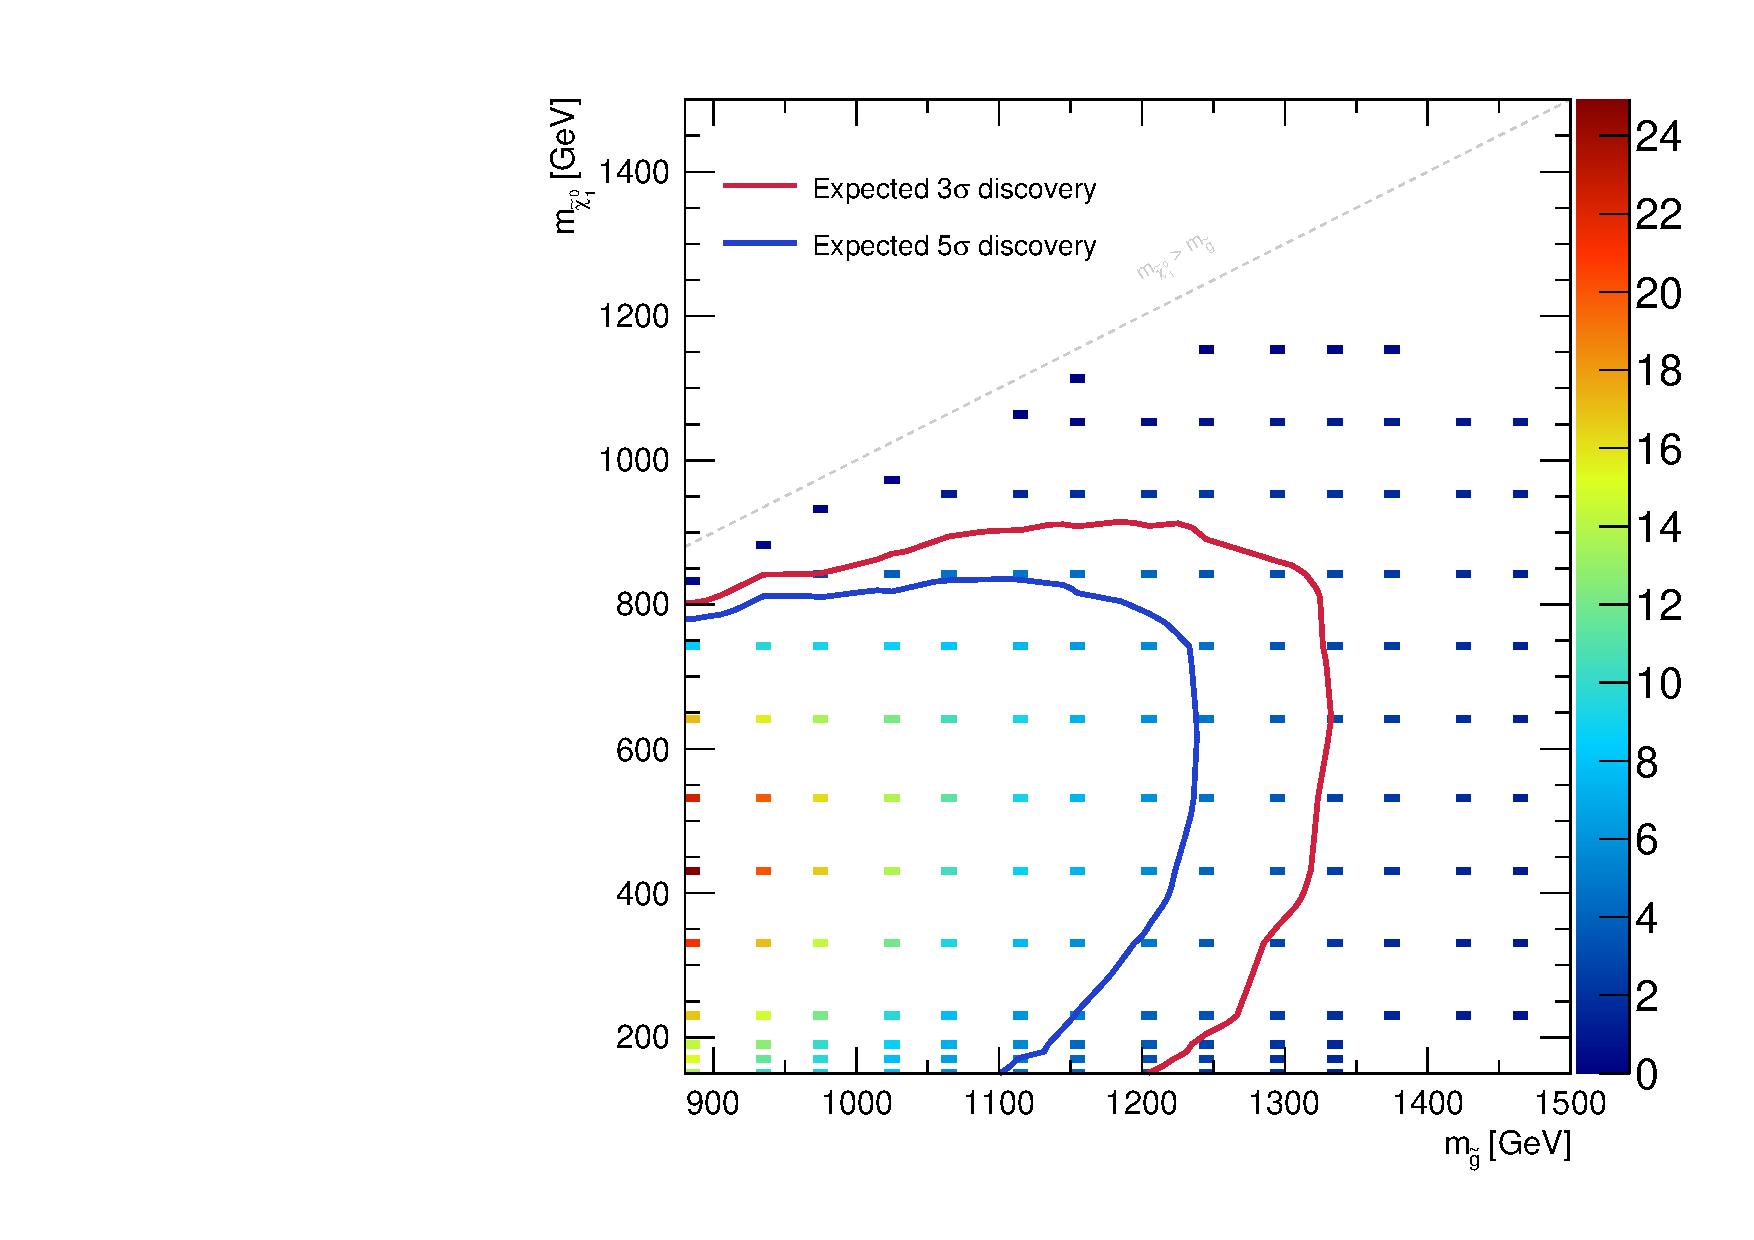
\includegraphics[width=0.49\textwidth]{discovery_srl_syst}
  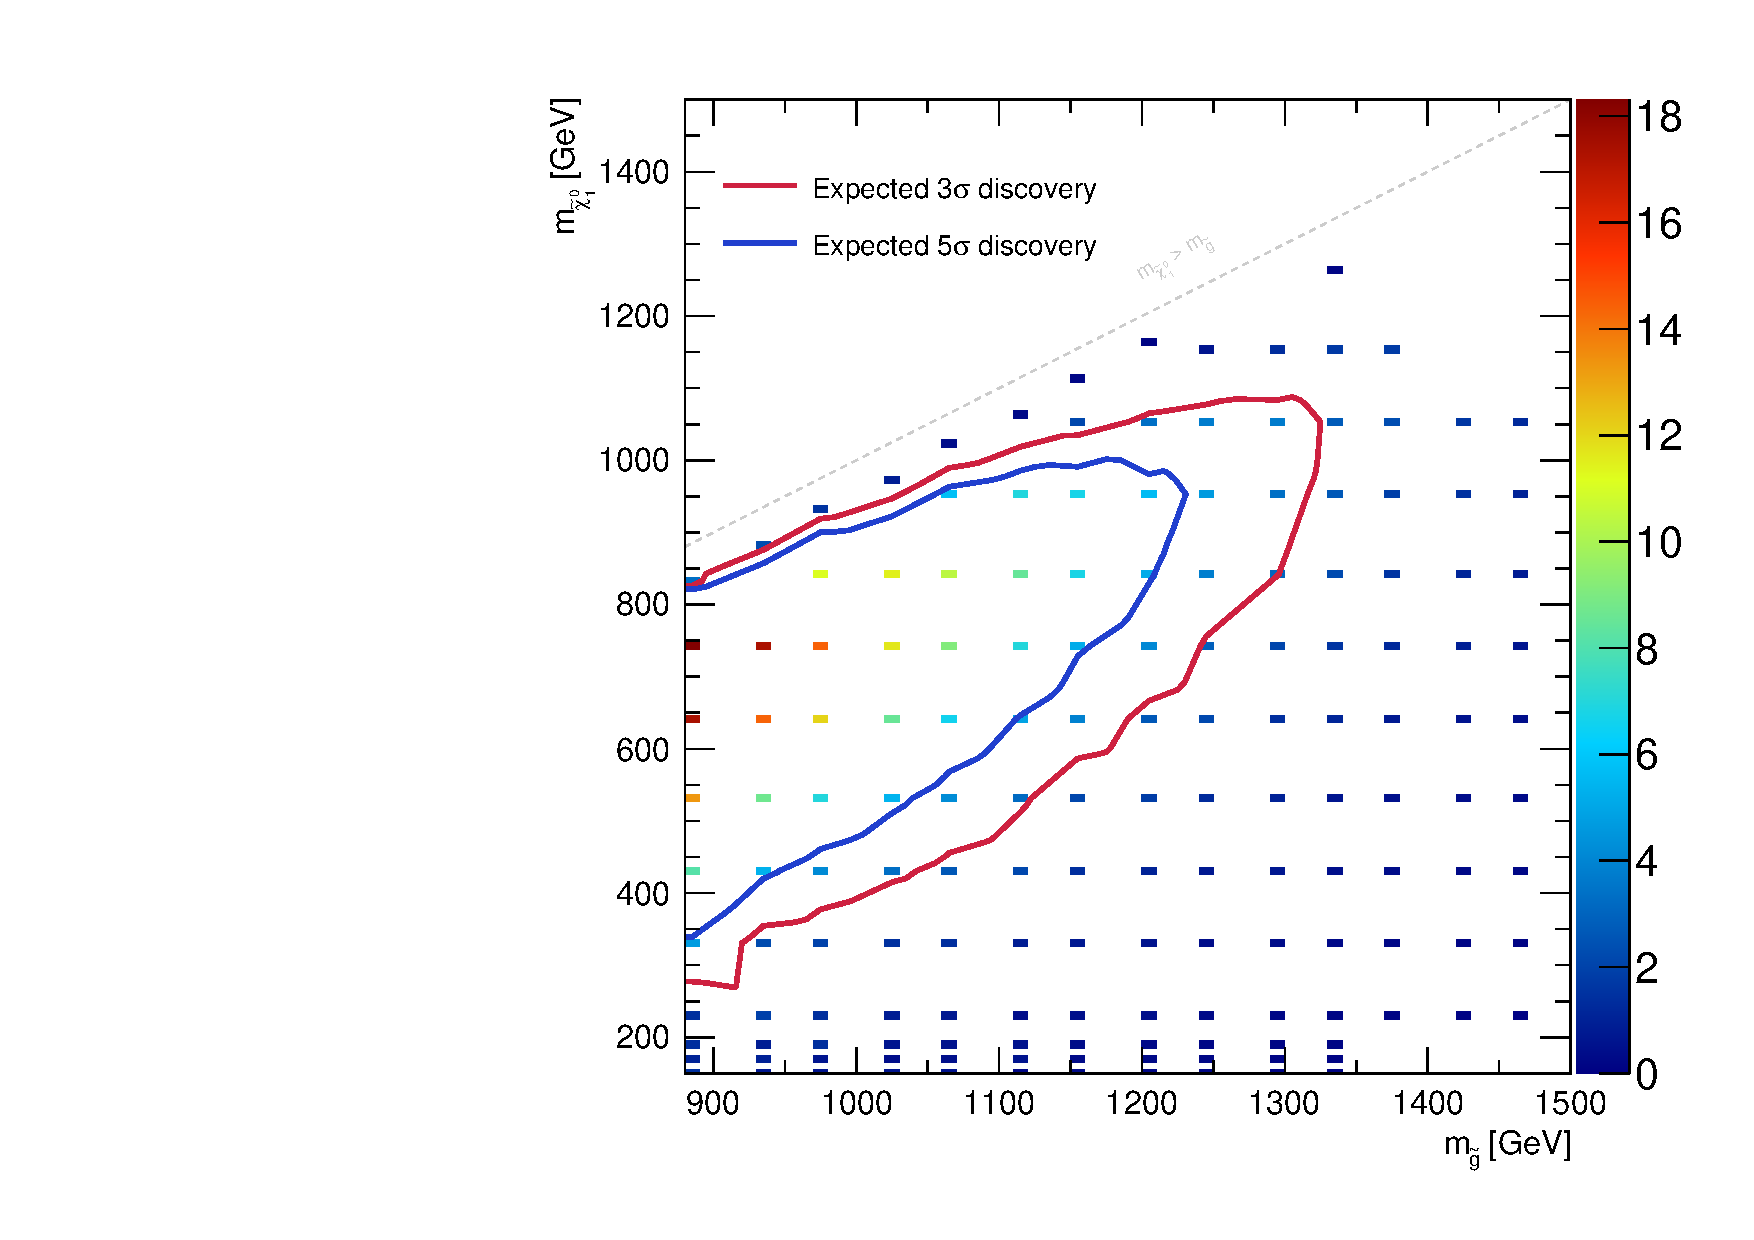
\includegraphics[width=0.49\textwidth]{discovery_srh_syst}

  \caption{Significancia de descubrimiento esperada para todos los puntos de la \emph{grid} de señal en el
    plano {\mgmn} para las dos regiones de señal {\SRL} (izquierda) y {\SRH} (derecha), junto
    con los contornos de $3\sigma$ y $5\sigma$.}

  \label{fig:opt_discovery_exp}
\end{figure}


\section{Aceptancia y eficiencia}

La aceptancia se define como:

\begin{equation}
  A = \frac{N_\mathrm{fiducial}}{N_\mathrm{total}}
\end{equation}
%
donde $N_\mathrm{fiducial}$ es el número de eventos que pasan los cortes
fiduciales basados en los objetos a nivel generador incluyendo los
cortes de {\pt} y $\eta$ del análisis. Además, se remueven los objetos
superpuestos en el espacio {\etaphi} como se describe en
\cref{sec:overlap_romoval_event_veto}. $N_\mathrm{total}$ es el número total
de eventos.

La eficiencia se define como:

\begin{equation}
  \epsilon = \frac{N_\mathrm{fiducial,reco}}{N_\mathrm{fiducial}}
\end{equation}
%
donde $N_\mathrm{fiducial,reco}$ es el número de eventos que pasan los cortes
nominales del análisis aplicados a las variables a nivel detector. La
eficiencia se diferencia de la aceptancia ya que incluye los efectos que provienen de
las ineficiencias de reconstrucción, los cortes de identificación de
partículas, y los efectos de resolución e ineficiencias del \emph{trigger}.

La aceptancia por la eficiencia ($A\times\epsilon$) fue calculada para las dos
regiones a partir de las muestras MC, para asegurar que en el proceso de
optimización se tuvieron en cuenta todas las regiones del espacio de parámetros,
y evitar caídas bruscas en la eficiencia de selección. En la
\cref{fig:atimeseff} se puede ver que hay una buena cobertura de toda la \emph{grid}
de señal.

\begin{figure}[!htb]
  \centering

  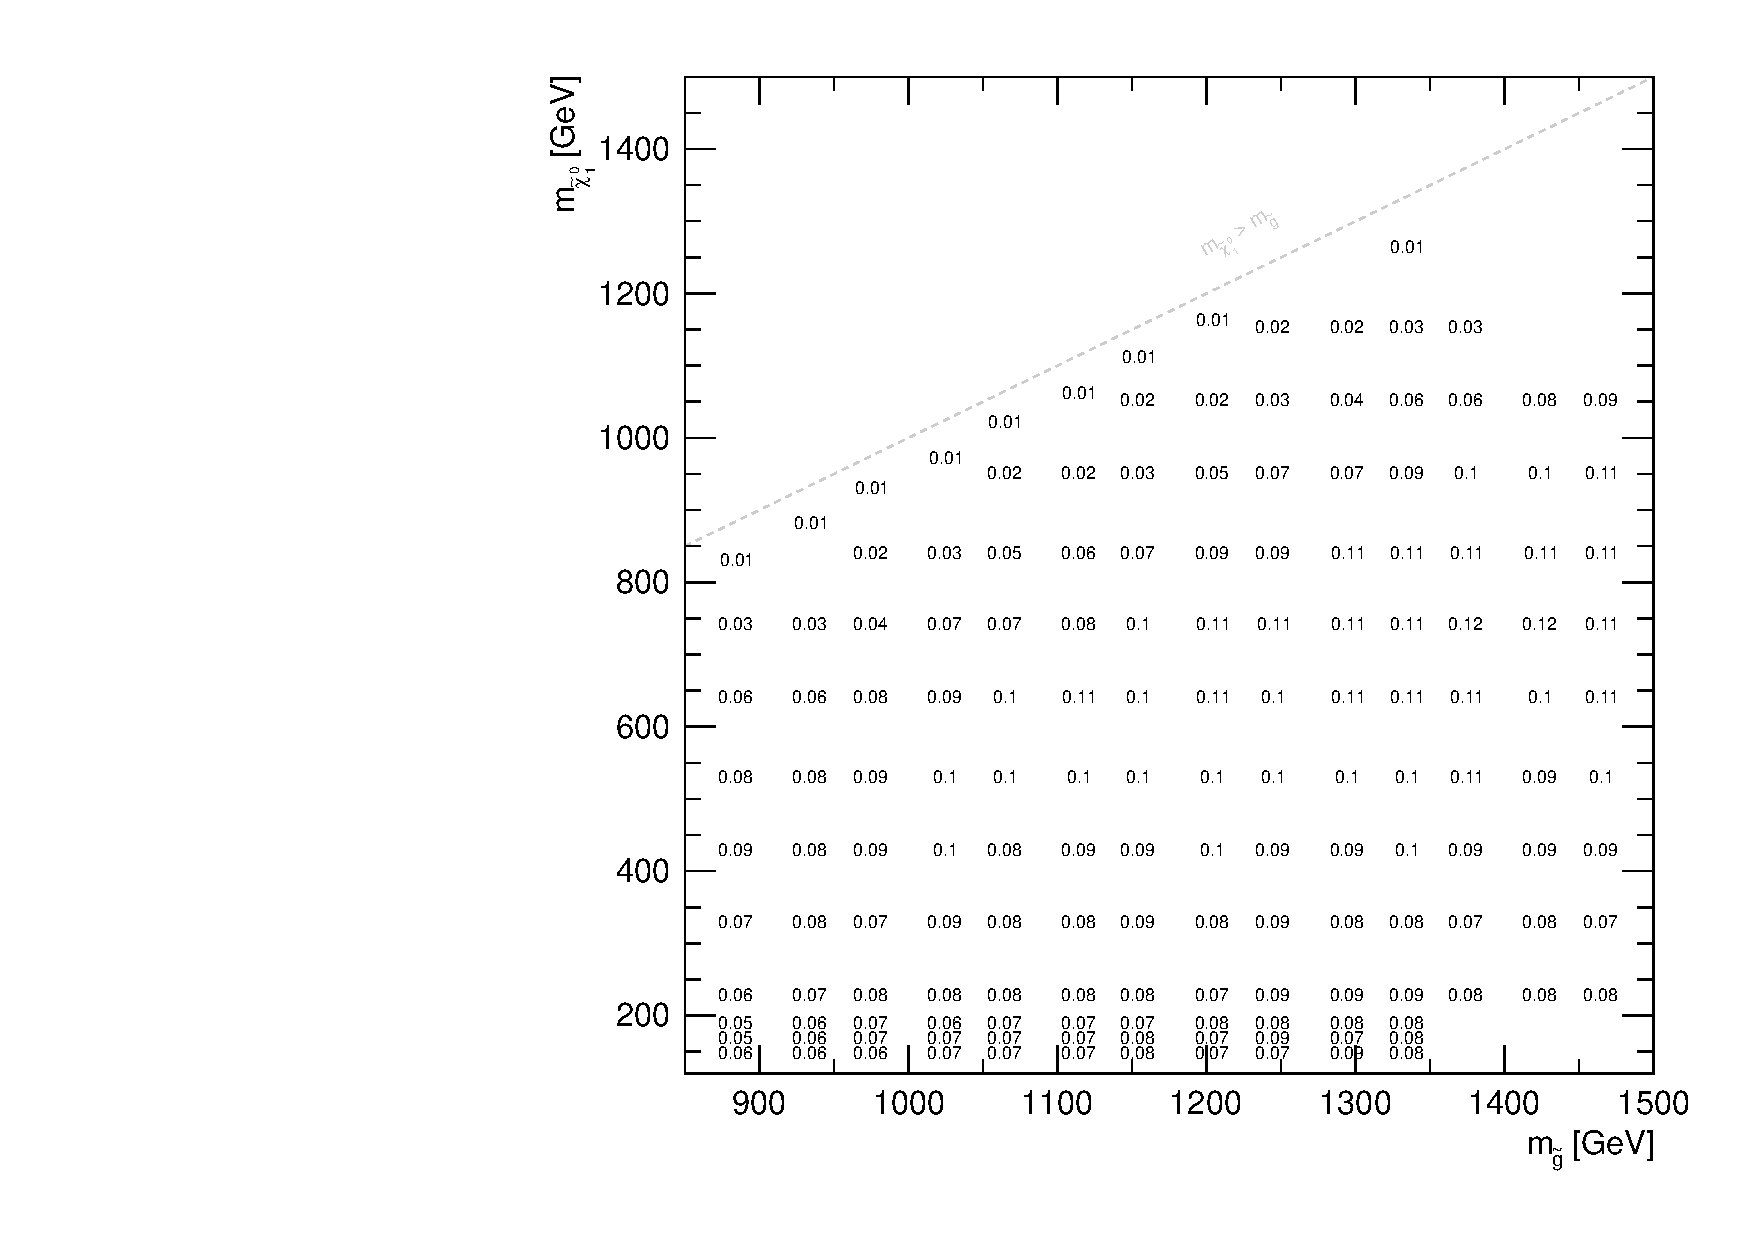
\includegraphics[width=0.45\textwidth]{acceptance_srl}
  \hspace{1cm}%
  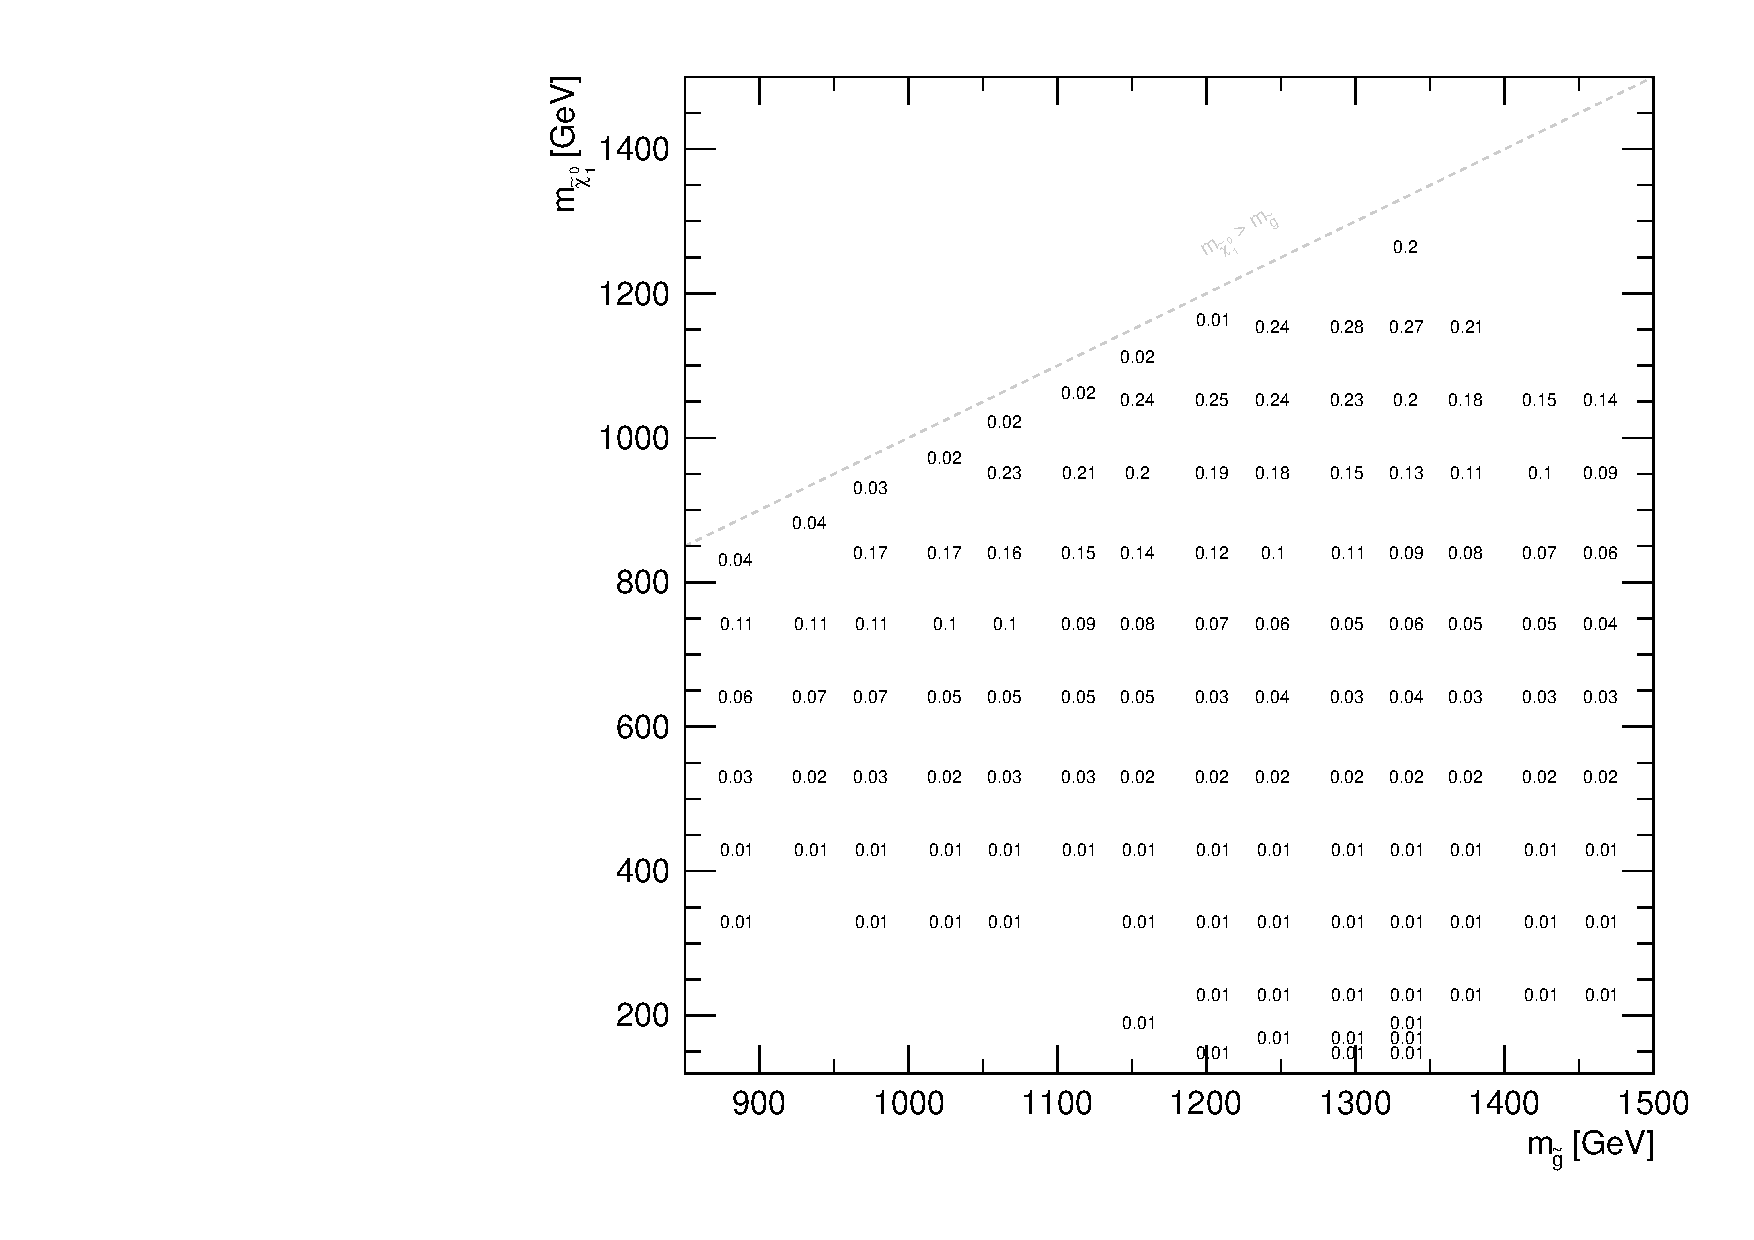
\includegraphics[width=0.45\textwidth]{acceptance_srh}

  \caption{Producto de la aceptancia y la eficiencia  ($A \times \epsilon$) de selección para cada punto de señal
    en el plano {\mgmn} para la {\SRL} (izquierda) y {\SRH} (derecha).}
  \label{fig:atimeseff}
\end{figure}
